% Options for packages loaded elsewhere
\PassOptionsToPackage{unicode}{hyperref}
\PassOptionsToPackage{hyphens}{url}
\documentclass[
  11pt,
]{article}
\usepackage{xcolor}
\usepackage[margin=22mm]{geometry}
\usepackage{amsmath,amssymb}
\setcounter{secnumdepth}{-\maxdimen} % remove section numbering
\usepackage{iftex}
\ifPDFTeX
  \usepackage[T1]{fontenc}
  \usepackage[utf8]{inputenc}
  \usepackage{textcomp} % provide euro and other symbols
\else % if luatex or xetex
  \usepackage{unicode-math} % this also loads fontspec
  \defaultfontfeatures{Scale=MatchLowercase}
  \defaultfontfeatures[\rmfamily]{Ligatures=TeX,Scale=1}
\fi
\usepackage{lmodern}
\ifPDFTeX\else
  % xetex/luatex font selection
\fi
% Use upquote if available, for straight quotes in verbatim environments
\IfFileExists{upquote.sty}{\usepackage{upquote}}{}
\IfFileExists{microtype.sty}{% use microtype if available
  \usepackage[]{microtype}
  \UseMicrotypeSet[protrusion]{basicmath} % disable protrusion for tt fonts
}{}
\makeatletter
\@ifundefined{KOMAClassName}{% if non-KOMA class
  \IfFileExists{parskip.sty}{%
    \usepackage{parskip}
  }{% else
    \setlength{\parindent}{0pt}
    \setlength{\parskip}{6pt plus 2pt minus 1pt}}
}{% if KOMA class
  \KOMAoptions{parskip=half}}
\makeatother
\usepackage{graphicx}
\makeatletter
\newsavebox\pandoc@box
\newcommand*\pandocbounded[1]{% scales image to fit in text height/width
  \sbox\pandoc@box{#1}%
  \Gscale@div\@tempa{\textheight}{\dimexpr\ht\pandoc@box+\dp\pandoc@box\relax}%
  \Gscale@div\@tempb{\linewidth}{\wd\pandoc@box}%
  \ifdim\@tempb\p@<\@tempa\p@\let\@tempa\@tempb\fi% select the smaller of both
  \ifdim\@tempa\p@<\p@\scalebox{\@tempa}{\usebox\pandoc@box}%
  \else\usebox{\pandoc@box}%
  \fi%
}
% Set default figure placement to htbp
\def\fps@figure{htbp}
\makeatother
\setlength{\emergencystretch}{3em} % prevent overfull lines
\providecommand{\tightlist}{%
  \setlength{\itemsep}{0pt}\setlength{\parskip}{0pt}}
\usepackage{bookmark}
\IfFileExists{xurl.sty}{\usepackage{xurl}}{} % add URL line breaks if available
\urlstyle{same}
\hypersetup{
  hidelinks,
  pdfcreator={LaTeX via pandoc}}

\author{}
\date{}

\newfontfamily\ReaderSymbols{seguisym.ttf}[Path=C:/Windows/Fonts/]
\begin{document}

\section{Elliptic complexes, diagonal traces, and fixed
points}\label{elliptic-complexes-diagonal-traces-and-fixed-points}

\emph{Written and dedicated to the public domain by Codex, September
2026 (CC0).}

An elliptic complex has a finite-dimensional space of harmonic
representatives even though its individual differentials may be
rectangular. That finite space makes an Euler index possible. A
commuting operator with a singular kernel can still have a trace along
the diagonal when its singular directions avoid the diagonal conormal.
The same chain homotopy then turns that distributional supertrace into a
cohomological one. For pullback by a smooth self-map, the trace becomes
a signed count of nondegenerate fixed points, including maps whose
derivative is singular.

The needed course results are
\href{geometric-microlocal-calculus.pdf}{Detecting regularity without
choosing coordinates} for bundle kernels, adjoints, wave fronts, and
controlled convergence; \href{global-elliptic-symbol-index.pdf}{Symbols,
finite defects, and the index on a closed manifold} for the full
elliptic alternative on every Sobolev scale; and
\href{traces-and-complexes.pdf}{Traces that survive passage to
cohomology} for finite-rank and graded trace algebra. We prove the extra
microlocal diagonal argument here. The chosen density, all half-density
factors, both Laplacian summands, source-to-target bundle maps, and
every determinant sign stay visible.

\subsection{1. The original complex and exactness of its
symbol}\label{the-original-complex-and-exactness-of-its-symbol}

Let \(X\) be a compact smooth manifold without boundary and let
\(E_0,\ldots,E_N\) be smooth finite-rank complex bundles. Give every
\(E_j\otimes\Omega_X^{1/2}\) a Hermitian metric and put
\(E_{-1}=E_{N+1}=0\). For one real order \(m\), retain each actual
bundle map \[
 D_j\in\Psi^m_{\mathrm{cl}}
   (X;E_j\otimes\Omega_X^{1/2},E_{j+1}\otimes\Omega_X^{1/2}),
 \quad -1\le j\le N,\qquad
 D_{-1}=D_N=0,\qquad D_jD_{j-1}=0.
 \tag{EC1}
\] Write \(d_j(x,\xi):E_{j,x}\to E_{j+1,x}\) for its homogeneous
principal symbol, with the original cotangent variable \(\xi\ne0\). The
symbol complex is elliptic exactly when \[
 \ker d_j(x,\xi)=\operatorname{ran}d_{j-1}(x,\xi)
 \quad(0\le j\le N,\ (x,\xi)\in T^*X\setminus0).
 \tag{EC2}
\] At the endpoints this includes injectivity of \(d_0\) and
surjectivity of \(d_{N-1}\); the zero bundles in (EC1) supply the exact
types. No rank equality between adjacent bundles is assumed. For the de
Rham example, fix a positive smooth density \(\mu\), take
\(E_j=\Lambda^jT^*X\), \(m=1\), and use the correctly typed half-density
differential \(D_j=M_{\mu^{1/2}}dM_{\mu^{-1/2}}\). Its original
principal symbol is \[
 d_j(x,\xi)\omega=i\,\xi\wedge\omega
 \quad\text{under }D=-i\partial.
 \tag{EC3}
\] The common nonzero factor \(i\) does not alter the kernel. To prove
exactness directly, choose \(v\in T_xX\) with \(\xi(v)=1\). Interior
multiplication obeys the exact identity
\(\iota_v(\xi\wedge\omega)+\xi\wedge\iota_v\omega=\omega\). If
\(\xi\wedge\omega=0\), then \(\omega=\xi\wedge\iota_v\omega\); at degree
zero this says the kernel is zero, and at top degree it proves
surjectivity. Thus (EC2) holds in every degree.

\subsection{2. The full Laplacian symbol and Hodge
representative}\label{the-full-laplacian-symbol-and-hodge-representative}

Choose the distributional Hermitian adjoints \(D_j^*\), preserving the
half-density bundle types, and define \[
 \Delta_j=D_{j-1}D_{j-1}^*+D_j^*D_j,\qquad
 \ell_j=d_{j-1}d_{j-1}^*+d_j^*d_j
       :E_j\longrightarrow E_j.
 \tag{EC4}
\] Both terms have order \(2m\). For every \(v\in E_{j,x}\), \[
 \langle\ell_jv,v\rangle
   =\|d_{j-1}^*v\|^2+\|d_jv\|^2.
 \tag{EC5}
\] If (EC2) holds and the right side vanishes, then \(v\in\ker d_j
=\operatorname{ran}d_{j-1}\) and \(v\perp\operatorname{ran}d_{j-1}\),
hence \(v=0\). Conversely, if \(\ell_j\) is injective for every \(j\),
decompose any \(v\in\ker d_j\) orthogonally in the finite-dimensional
fiber as \(v=v_{\mathrm{ran}}+v_\perp\) with
\(v_{\mathrm{ran}}\in\operatorname{ran}d_{j-1}\) and
\(v_\perp\perp\operatorname{ran}d_{j-1}\). The complex identity gives
\(d_jv_{\mathrm{ran}}=0\), so \(d_jv_\perp=0\), and
\(d_{j-1}^*v_\perp=0\); (EC5) makes \(v_\perp=0\). Thus (EC2) is
equivalent to ellipticity of every complete \(\Delta_j\), without
deleting either summand.

Elliptic Fredholm theory in the current owned global-index lesson
applies to \(\Delta_j:H^{s+2m}(E_j)\to H^s(E_j)\) for every real \(s\).
Its kernel is smooth and finite dimensional. For a smooth kernel
element, the integrated version of (EC5) shows that this kernel is
exactly \[
 K_j=\ker D_j\cap\ker D_{j-1}^*
     =\ker\Delta_j\subset C^\infty(X;E_j\otimes\Omega_X^{1/2}).
 \tag{EC6}
\] Fix an \(L^2\)-orthonormal basis \(k_{j,1},\ldots,k_{j,r_j}\) of
\(K_j\) and keep the full finite-rank projection \[
 H_j f=\sum_{\alpha=1}^{r_j}
             \langle f,k_{j,\alpha}\rangle\,k_{j,\alpha}.
 \tag{EC7}
\] For a distribution \(f\), the bracket is its distribution-smooth
pairing with \(k_{j,\alpha}\); \(H_j\) has a smooth kernel and acts
coherently on every Sobolev order. If \(r_j=0\), the sum is zero.

The adjoint kernel of \(\Delta_j:H^{s+2m}\to H^s\) is the same smooth
\(K_j\), with its correct anti-dual Sobolev realization. Its range is
the annihilator of \(K_j\), by the exact elliptic alternative. Therefore
\[
 \Delta_j+H_j:H^{s+2m}(E_j)\xrightarrow{\;\cong\;}H^s(E_j)
 \quad\text{for every }s.
 \tag{EC8}
\] For surjectivity, split \(f=(f-H_jf)+H_jf\); the first summand
annihilates \(K_j\) and is \(\Delta_jg_0\). Replace \(g_0\) by
\(g_0-H_jg_0\) and add \(H_jf\). For injectivity, pair
\((\Delta_j+H_j)g=0\) with each \(k_{j,\alpha}\) to get \(H_jg=0\), and
then \(\Delta_jg=0\) gives \(g\in K_j\), hence \(g=0\). The bounded
inverse theorem applies to the displayed Banach isomorphism. This
argument uses \(\Delta_j\) with its original order \(2m\); it does not
assume \(m>0\) or an \(L^2\) inverse for a negative-order operator.

Let \[
 F_j=(\Delta_j+H_j)^{-1}(I-H_j)
      =(\Delta_j+H_j)^{-1}-H_j.
 \tag{EC9}
\] The second equality follows because \((\Delta_j+H_j)H_j=H_j\). The
full elliptic parametrix of \(\Delta_j+H_j\) has order \(-2m\), and the
difference from its actual inverse is smoothing: if \(B_j\) is one
parametrix, then \((\Delta_j+H_j)^{-1}
 =B_j+(\Delta_j+H_j)^{-1}(I-(\Delta_j+H_j)B_j)\); the second term maps
every Sobolev order to every higher order, and applying the
corresponding adjoint identity gives the same bound in the input
variable, hence a smooth kernel. Thus \(F_j\in\Psi^{-2m}\), with exact
identities \[
 \Delta_jF_j=F_j\Delta_j=I-H_j,\qquad
 F_jH_j=H_jF_j=0.
 \tag{EC10}
\] The range of \(F_j\) is in the annihilator of \(K_j\). These
operators agree on all Sobolev realizations by uniqueness in (EC8).

The complex identity proves the exact intertwining, retaining both
Laplacian summands: \[
 D_j\Delta_j
  =D_jD_j^*D_j
  =\Delta_{j+1}D_j,\qquad
 D_jH_j=H_{j+1}D_j=0,\qquad
 D_jF_j=F_{j+1}D_j.
 \tag{EC11}
\] For the last equality, intertwine \(\Delta+H\) and its actual
inverse, then multiply by \(I-H\). Adjoints give
\(D_j^*F_{j+1}=F_jD_j^*\).

\subsection{3. The exact pseudodifferential chain homotopy, its
smoothing remainder, and
cohomology}\label{the-exact-pseudodifferential-chain-homotopy-its-smoothing-remainder-and-cohomology}

With the endpoint convention \(G_{-1}=G_N=0\), define the
degree-lowering maps \[
 G_j=D_j^*F_{j+1}=F_jD_j^*:
    \mathcal D'(E_{j+1})\longrightarrow\mathcal D'(E_j),
 \qquad G_j\in\Psi^{-m}.
 \tag{EC12}
\] Equation (EC11) retains the factor order needed to compute \[
 D_{j-1}G_{j-1}+G_jD_j
  =(D_{j-1}D_{j-1}^*+D_j^*D_j)F_j
  =I-H_j.
 \tag{EC13}
\] Thus \(H_j=I-D_{j-1}G_{j-1}-G_jD_j\) is the actual smooth-kernel
chain homotopy remainder; it commutes with the differential because both
\(D_jH_j\) and \(H_{j+1}D_j\) vanish. It induces the identity on
cohomology.

For every \(s\in\mathbb R\), if \(f\in H^s(E_j)\) and \(D_jf=0\)
distributionally, (EC13) gives \[
 f=H_jf+D_{j-1}(G_{j-1}f),\qquad
 G_{j-1}f\in H^{s+m}(E_{j-1}).
 \tag{EC14}
\] The exact Sobolev shift is \(s+m\), since \(G_{j-1}\) has order
\(-m\). The harmonic part is the unique representative of the cohomology
class: if a harmonic \(k\) equals \(D_{j-1}v\) for a distribution \(v\),
then \(\langle k,k\rangle=\langle v,D_{j-1}^*k\rangle=0\), where
elliptic regularity first makes \(k\) smooth, so \(k=0\). Conversely the
difference between a closed \(f\) and \(H_jf\) has the explicit
primitive in (EC14). Smooth input has a smooth primitive because
\(G_{j-1}\) preserves smooth sections. Every distribution belongs to
some \(H^s\) on compact \(X\), so the same statement holds for the full
distributional complex. Therefore smooth, Sobolev and distributional
cohomology in degree \(j\) are all canonically \(K_j\), of finite
dimension \(r_j\).

The Sobolev complex in that statement has its exact degree shifts. For
each fixed real \(t\), put \[
 \begin{aligned}
 \mathcal H^j_t&=H^{t-jm}(X;E_j\otimes\Omega_X^{1/2}),&
 D_j&:\mathcal H^j_t\longrightarrow\mathcal H^{j+1}_t,\\
 \frac{\ker(D_j:\mathcal H^j_t\to\mathcal H^{j+1}_t)}
      {D_{j-1}\mathcal H^{j-1}_t}
 &\ \xrightarrow{\ [f]\mapsto H_jf\ }\ K_j.&
 \end{aligned}
 \tag{EC14a}
\] The denominator is contained in the numerator by \(D_jD_{j-1}=0\). It
is exactly the subspace \(\{f\in\mathcal H^j_t:D_jf=0,\ H_jf=0\}\): one
inclusion follows from \(H_jD_{j-1}=0\), and the other follows from
(EC14), whose primitive lies in \(H^{t-jm+m}=\mathcal H^{j-1}_t\). Both
equations defining this subspace are continuous on \(\mathcal H^j_t\),
so the boundary space is closed. Consequently the quotient is a
finite-dimensional Hausdorff space, and the displayed map and its
inverse \(k\mapsto[k]\) are continuous. The inclusions from smooth
sections and into distributions commute with these maps because the
actual \(H_j\) and \(G_j\) agree on all realizations. This gives the
precise canonical comparison, including every negative, zero and
positive differential order \(m\).

Let \(D=\sum_j D_j\) on the graded sum \(\bigoplus_j E_j\), and
\(A=D+D^*\), with its actual even-to-odd component \(A_{\mathrm{ev}}\).
The full square \(A^2=\bigoplus_j\Delta_j\), since \(D^2=(D^*)^2=0\).
Its principal symbol square is \(\bigoplus_j\ell_j\), so
\(A_{\mathrm{ev}}\) is elliptic. The even kernel is
\(\bigoplus_{j\ \mathrm{even}}K_j\), and the adjoint odd kernel is
\(\bigoplus_{j\ \mathrm{odd}}K_j\), by the integrated energy identity.
Hence \[
 \chi(D_\bullet)=\sum_{j=0}^N(-1)^j\dim K_j
     =\operatorname{ind}A_{\mathrm{ev}}.
 \tag{EC15}
\] No Fredholm index is assigned to an individual rectangular \(D_j\)
merely because the whole symbol sequence is exact.

\subsection{4. Diagonal traces for singular kernels and the required
cyclicity}\label{diagonal-traces-for-singular-kernels-and-the-required-cyclicity}

Write \(\Delta_X=\{(x,x):x\in X\}\subset X\times X\). For a continuous
map \(R:C^\infty(X;E)\to\mathcal D'(X;E)\), its distributional Schwartz
kernel \(K_R\) is a section of the output-input bundle with the input
density factor. The diagonal trace is defined when \[
 \operatorname{WF}(K_R)\cap
 N^*\Delta_X=\varnothing,\qquad
 N^*\Delta_X
 =\{(x,x;\xi,-\xi):\xi\in T_x^*X\setminus0\}.
 \tag{EC16}
\] Indeed, the pullback \(\Delta_X^*K_R\) then exists as a
distributional density on \(X\). Its fiber trace is a density, and
compactness permits the exact scalar \[
 \operatorname{Tr}_{\Delta_X}R
    =\int_X\operatorname{tr}_E(\Delta_X^*K_R).
 \tag{EC17}
\] The finite chart proof of this pullback is Fourier restriction: in
coordinates near the diagonal, a test of the pullback requires
integrating the full Fourier transform along the normal-frequency
directions \((\xi,-\xi)\). Condition (EC16) gives rapid decay in a cone
containing those directions, while polynomial distribution bounds handle
the complementary compact-frequency part. Cutoffs and changes of
coordinates preserve the condition and give the same distribution. This
construction retains the actual density and bundle trace, not merely a
formal value \(K_R(x,x)\).

We need two continuity facts and prove the estimates that matter. Let a
compactly localized kernel \(K\) have wave front disjoint from
\(N^*\Delta_X\). In a chart-product cutoff, convolve \(K\) with a smooth
approximate identity in both variables, or multiply its full Fourier
transform by a compactly supported multiplier
\(\rho(\varepsilon(\xi,\eta))\) equal to one near zero. The resulting
smooth \(K_\varepsilon\) tends to \(K\) weakly. On any closed cone
disjoint from \(\operatorname{WF}(K)\), all localized Fourier transforms
of \(K\) decrease faster than every power. The multiplier is uniformly
bounded; for a fixed weighted rapid-decay seminorm split at radius
\(L\), use pointwise convergence on the bounded part and a stronger
rapid-decay bound \(C_ML^{N-M}\) on the tail. Thus \[
 K_\varepsilon\longrightarrow K
 \quad\text{in every wave-front-topology seminorm on cones
 disjoint from }\operatorname{WF}(K).
 \tag{EC18}
\] Finite chart partitions and smoothing off-diagonal overlaps give a
global smoothing family with the same property.

Let \(A\in\Psi^r(X)\) be properly supported. The statement needed here
concerns a cone around \(N^*\Delta_X\), where both output and input
covectors are nonzero. A pseudodifferential kernel can be split into a
part supported in an arbitrarily small neighborhood of its diagonal and
a smooth remainder. For the first part, output composition has a
localized full Fourier transform given by an integral in an intermediate
output frequency \(\xi'\); the Fourier transform in \(x\) of its
smooth-symbol coefficient decreases faster than any power of
\(|\xi-\xi'|\), with at most a fixed polynomial factor in \(|\xi'|\).
Split into \(|\xi-\xi'|\le c|(\xi,\eta)|\) and its complement. In the
first region, a smaller conic neighborhood of the diagonal conormal
stays inside a larger one, so use the arbitrary rapid-decay bound
supplied by (EC16). In the complement, the rapidly decreasing
coefficient absorbs the polynomial distribution bound and every
requested output power. The input-composition calculation is the same in
\(\eta\).

The smooth remainder of \(A\) needs a separate check: after output
composition it can retain a singular input covector, but its output
covector is zero; after input composition the reverse holds. Neither
one-sided direction meets \(N^*\Delta_X\). In particular the stronger
assertion that either composition preserves the \emph{entire} wave front
of \(K\) would be false. The exact two-sided inclusion that follows from
the near-diagonal calculation is \[
 \begin{aligned}
 \operatorname{WF}(AK)\cap T^*_{\ne0,\ne0}(X\times X)
   &\subseteq \operatorname{WF}(K),\\
 \operatorname{WF}(KA)\cap T^*_{\ne0,\ne0}(X\times X)
   &\subseteq \operatorname{WF}(K),
 \end{aligned}
 \quad
 T^*_{\ne0,\ne0}
  =\{(x,y;\xi,\eta):\xi\ne0,\ \eta\ne0\}.
 \tag{EC19}
\] The same split, with the uniform bounds in (EC18), proves convergence
of the composed smooth approximants in the conic seminorms around
\(N^*\Delta_X\). Consequently (EC16) holds for \(AK\) and \(KA\), and
their diagonal traces converge. We claim no preservation of the
wave-front seminorms at one-sided directions. To see why the restriction
is necessary, take a circle, a point \(y_0\), and smooth functions
\(f,g,h\) with
\(\operatorname{supp}f\cap\operatorname{supp}g=\varnothing\) and
\(\int hf\ne0\). Put \(K(z,y)=f(z)\delta(y-y_0)\) and let \(A\) have the
smooth rank-one kernel \(g(x)h(z)\). Then
\(AK(x,y)=(\int hf)g(x)\delta(y-y_0)\), which has input-only wave-front
directions over \(\operatorname{supp}g\times\{y_0\}\) where \(K\) has
none. Both kernels remain transverse to \(N^*\Delta_X\), exactly as
(EC19) requires.

For any \(A\in\Psi^r(E,F)\) and kernel map \(B:F\to E\) satisfying
(EC16) in the corresponding typed compositions, these facts give the
exact microlocal cyclicity \[
 \operatorname{Tr}_{\Delta_X}(AB)
       =\operatorname{Tr}_{\Delta_X}(BA).
 \tag{EC20}
\] To verify it without treating \(A\) as bounded on \(L^2\), use the
smooth approximants \(B_\varepsilon\). Both \(AB_\varepsilon\) and
\(B_\varepsilon A\) have smooth kernels. Expand \(B_\varepsilon\) in a
finite Fourier-basis approximation, whose smooth-kernel remainder tends
to zero in every smooth seminorm; for each finite-rank term the
distributional adjoint identity gives equality of the two traces. The
smooth-kernel remainder is trace-norm small after applying \(A\),
because its double Fourier coefficients decrease faster than the
polynomial matrix growth of \(A\). Thus the trace equality holds for
\(B_\varepsilon\). The continuity just proved sends both sides to
(EC20). Fiber types and matrix trace are retained by the finite-rank
identity.

\subsection{5. Supertrace of a commuting distributional chain
map}\label{supertrace-of-a-commuting-distributional-chain-map}

Let \(R_j:C^\infty(E_j)\to\mathcal D'(E_j)\) be continuous for every
\(j\), assume \[
 D_jR_j=R_{j+1}D_j
 \quad\text{on smooth sections,}\qquad
 \operatorname{WF}(K_{R_j})\cap N^*\Delta_X=\varnothing.
 \tag{EC21}
\] The chain identity extends by continuity where compositions of
distributions are defined. A closed smooth \(f\) maps to a closed
distribution, so (EC14) defines its action on cohomology. The induced
finite-dimensional map on \(K_j\) is \(H_jR_j|_{K_j}\). Since \(H_j\)
has a smooth finite-rank kernel, \(H_jR_jH_j\) has a smooth finite-rank
kernel and \[
 \operatorname{Tr}(H_jR_jH_j)
       =\operatorname{Tr}_{K_j}(H_jR_j|_{K_j}).
 \tag{EC22}
\]

To compare it with the singular-kernel diagonal trace, retain the
degree-lowering operator in both terms: \[
 L_j=G_{j-1}R_j+H_{j-1}R_{j-1}G_{j-1}:E_j\to E_{j-1}.
 \tag{EC23}
\] Using (EC13), the chain identity (EC21), \(D_{j-1}H_{j-1}=0\), and
\(H_jR_jD_{j-1}=H_jD_{j-1}R_{j-1}=0\), calculate in its actual order \[
 \begin{aligned}
 D_{j-1}L_j+L_{j+1}D_j
 &= (D_{j-1}G_{j-1}+G_jD_j)R_j
       +H_jR_jG_jD_j\\
 &= (I-H_j)R_j+H_jR_j(I-H_j)\\
 &=R_j-H_jR_jH_j.
 \end{aligned}
 \tag{EC24}
\] Each kernel appearing on the right and in the first line has a
diagonal trace. For \(G R\) and \(R G\), this follows from (EC19) and
the original (EC21); for a term with \(H\), one side is smooth and
cannot have a nonzero diagonal conormal in both variables. Apply (EC20)
to \(D_j\) and \(L_{j+1}\), sum (EC24) with the original alternating
signs, and reindex only after all source and target types are fixed: \[
 \begin{aligned}
 \sum_j(-1)^j\operatorname{Tr}_{\Delta_X}
       (R_j-H_jR_jH_j)
 &=\sum_j(-1)^j
      \bigl(\operatorname{Tr}_{\Delta_X}(D_{j-1}L_j)
           +\operatorname{Tr}_{\Delta_X}(L_{j+1}D_j)\bigr)\\
 &=\sum_j\bigl((-1)^{j+1}+(-1)^j\bigr)
        \operatorname{Tr}_{\Delta_X}(L_{j+1}D_j)=0.
 \end{aligned}
 \tag{EC25}
\] The endpoint maps in (EC1) make the dropped end terms exactly zero.
Equations (EC22)--(EC25) prove the full supertrace identity \[
 \sum_{j=0}^N(-1)^j\operatorname{Tr}_{\Delta_X}R_j
 =\sum_{j=0}^N(-1)^j
      \operatorname{Tr}_{K_j}(H_jR_j|_{K_j}).
 \tag{EC26}
\] This is an equality of a distributional diagonal trace and the actual
induced cohomology trace, not an assertion that each nonsmoothing
\(R_j\) is trace class.

\subsection{6. The vanishing high-frequency tail used in diagonal
limits}\label{the-vanishing-high-frequency-tail-used-in-diagonal-limits}

The controlled-kernel argument also gives the exact vanishing-parametrix
statement. Let \(a_\varepsilon(x,\xi)\) be bounded in every symbol
seminorm of one fixed \(S^r\) class and tend to zero with all
derivatives on each compact \((x,\xi)\) set. Its quantized kernels have
wave front contained in \(N^*\Delta_X\), converge to zero weakly, and
converge to zero in every wave-front-topology seminorm on cones outside
\(N^*\Delta_X\): \[
 K_{\operatorname{Op}(a_\varepsilon)}
 \longrightarrow0
 \quad\text{in }\mathcal D'(X\times X)
 \text{ and in the controlled topology off }N^*\Delta_X.
 \tag{EC27}
\] For weak convergence, pair the oscillatory kernel with a compact
smooth test, take its Fourier transform in \(x-y\), and use the test's
arbitrary rapid decay against the uniform polynomial symbol bound;
pointwise convergence then gives dominated convergence. Away from
\(N^*\Delta_X\), the finite-chart kernel estimate from the owned
geometric microlocal lesson gives \(C_M\langle(\xi,\eta)\rangle^{-M}\)
uniformly for every \(M\). On bounded frequencies use the already-proved
weak convergence of localized kernels; on the tail choose \(M\) larger
than the requested weighted seminorm. This proves (EC27), including all
chart and cutoff derivatives.

For a concrete high-frequency tail, take the full symbol
\(f_j(x,\xi)\in S^{-2m}\) of \(F_j\) in each fixed chart and a smooth
radial scalar \(\chi\) which is zero near the origin and one outside a
larger ball. Use the fixed cotangent metric and the same chart partition
in every member of the family. Define the localized symbols and their
patched operator by \[
 f_{j,\varepsilon}(x,\xi)
   =\chi(\varepsilon\xi)f_j(x,\xi),\qquad
 F_{j,\varepsilon}=\operatorname{Op}(f_{j,\varepsilon}).
 \tag{EC28}
\] For fixed \(\xi\), every derivative tends to zero as
\(\varepsilon\downarrow0\). Each cutoff derivative
\(\varepsilon^{|\beta|}\partial^\beta\chi(\varepsilon\xi)\) is supported
where \(|\xi|\asymp\varepsilon^{-1}\) and has the exact
\(\langle\xi\rangle^{-|\beta|}\) symbol cost, so the family is uniformly
bounded in \(S^{-2m}\). Formula (EC27) applies for every real \(m\).

Here is the needed trace-limit argument with both conic factors
retained. After a finite partition of unity on \(X\times X\), the trace
of \(R F_{j,\varepsilon}\) is the distributional pairing of \(K_R(x,z)\)
with the transposed kernel \(K_{F_{j,\varepsilon}}(z,x)\), including the
bundle composition and both density factors. The pairing is defined
because the second wave front is contained in the diagonal conormal and
(EC16) excludes its negative from the first. In Fourier coordinates,
divide the frequency integral into a closed cone around that conormal
and its complement. On the first cone, the localized transform of
\(K_R\) has arbitrary rapid decay, while the transform of
\(K_{F_{j,\varepsilon}}\) has a uniform polynomial bound from its
\(S^{-2m}\) seminorms. On the complementary closed cone, the latter has
uniform arbitrary rapid decay by (EC27), while the former has a fixed
polynomial distribution bound. Choose the rapid-decay powers greater
than the respective polynomial powers plus \(2\dim X+1\); both products
then have an integrable majorant. The localized transforms of
\(K_{F_{j,\varepsilon}}\) tend pointwise to zero by weak convergence in
(EC27), so dominated convergence makes every localized pairing tend to
zero. The same proof with the kernels in reverse order treats
\(F_{j,\varepsilon}R\). Consequently \[
 \operatorname{Tr}_{\Delta_X}(R F_{j,\varepsilon})
       \longrightarrow0,\qquad
 \operatorname{Tr}_{\Delta_X}(F_{j,\varepsilon} R)
       \longrightarrow0.
 \tag{EC29}
\] Proper cutoffs obey the same cone split. If a chosen representation
of \(F_j\) also has a smoothing remainder, apply the same high-frequency
cutoff to a rapidly decreasing complete symbol for each compactly
localized piece of that remainder; those tails tend to zero in every
smooth-kernel seminorm. An unchanged smoothing remainder is not part of
\(F_{j,\varepsilon}\). This establishes the high-frequency tail removal
used in the diagonal-trace route while (EC24) supplies a direct exact
homotopy identity.

\subsection{7. The full noninvertible-map fixed-point
calculation}\label{the-full-noninvertible-map-fixed-point-calculation}

Choose a Riemannian metric and keep the positive smooth density \(\mu\)
fixed in (EC3). In the de Rham complex, let \(\phi:X\to X\) be any
smooth map; no inverse or local diffeomorphism is assumed. The ordinary
pullback on \(j\)-forms is a chain map because \(d\phi^*=\phi^*d\), by
the coordinate chain rule. Conjugate it by the same multiplication with
\(\mu^{1/2}\) used for \(D_j\), so \(D_jR_j=R_{j+1}D_j\) has the exact
half-density types: \[
 R_j=M_{\mu^{1/2}}\circ\phi^*
                    \circ M_{\mu^{-1/2}}.
 \tag{EC30}
\] In one coordinate chart, its kernel coefficient relative to the input
coordinate density is exactly \[
 K_{R_j}(x,y)
 =\left(\frac{\mu(x)}{\mu(\phi(x))}\right)^{1/2}
   \Lambda^j(d\phi_x)^*\,\delta(y-\phi(x)).
 \tag{EC31}
\] The quotient of densities is evaluated in the chosen coordinate
trivialization, and on the diagonal at a fixed point it equals one. The
graph map \(x\mapsto(x,\phi(x))\) is an embedding even when \(d\phi_x\)
is singular, because its first component is the identity. Thus the delta
kernel has wave front contained in its graph conormal: \[
 \operatorname{WF}(K_{R_j})\subset
 \{(x,\phi(x);-d\phi_x^{\,T}\eta,\eta):
                      \eta\in T^*_{\phi(x)}X\setminus0\}.
 \tag{EC32}
\] The smooth matrix and density factor can only remove, not add, those
directions. At a fixed point \(x=\phi(x)\), intersection with
\(N^*\Delta_X\) requires \((-d\phi_x^T\eta,\eta)=(\xi,-\xi)\). Hence
\(d\phi_x^T\eta=\eta\). The exact transversality condition is therefore
\[
 \det(I-d\phi_x)\ne0
 \quad\text{at every fixed point }x.
 \tag{EC33}
\] This condition makes (EC16) hold for all \(R_j\). It also makes each
zero of the local map \(F(x)=x-\phi(x)\) isolated by the inverse
function theorem. The fixed set is closed in compact \(X\), hence is
finite.

At each fixed point \(x_\alpha\), the standard delta change-of-variables
formula, applied to the actual map \(F\) with its full Jacobian, gives
\[
 \delta(x-\phi(x))
   =\sum_\alpha
       \frac{\delta(x-x_\alpha)}
            {|\det(I-d\phi_{x_\alpha})|}.
 \tag{EC34}
\] To verify it, choose disjoint small neighborhoods on which \(F\) is a
diffeomorphism, test against a compact smooth function, change variables
\(z=F(x)\), and evaluate the Jacobian at \(z=0\). Outside those
neighborhoods the delta has no support. The density ratio in (EC31)
becomes one at each \(x_\alpha\); no Jacobian from a nonexistent inverse
of \(\phi\) is introduced.

Because \(\phi(x_\alpha)=x_\alpha\), the fiber map
\((d\phi_{x_\alpha})^*\) acts on the same cotangent space and has a
trace. Summing the complete exterior algebra, including degree zero and
top degree, gives \[
 \sum_{j=0}^{\dim X}(-1)^j
     \operatorname{tr}\Lambda^j((d\phi_{x_\alpha})^*)
 =\det(I-(d\phi_{x_\alpha})^*)
 =\det(I-d\phi_{x_\alpha}).
 \tag{EC35}
\] For a diagonalizable matrix this is the product
\(\prod_i(1-\lambda_i)\) by expanding it over all subsets of
eigenvalues. Both sides are polynomial in the matrix entries, and
diagonalizable complex matrices are dense, so the identity holds for
every matrix. The second determinant equality follows from equality of a
matrix and its transpose determinants, without assuming \(d\phi\) is
invertible.

Now apply the proved supertrace identity (EC26) to the chain map (EC30),
and evaluate its diagonal traces with (EC31)--(EC35). If \(L(\phi)\) is
the original alternating trace of \(\phi^*\) on de Rham cohomology, then
\[
 \begin{aligned}
 L(\phi)
 &=\sum_j(-1)^j
       \operatorname{Tr}\bigl(\phi^*:H^j_{\mathrm{dR}}(X)\to
                                    H^j_{\mathrm{dR}}(X)\bigr)\\
 &=\sum_\alpha
       \frac{\det(I-d\phi_{x_\alpha})}
            {|\det(I-d\phi_{x_\alpha})|}\\
 &=\sum_{\phi(x_\alpha)=x_\alpha}
         \operatorname{sgn}\det(I-d\phi_{x_\alpha}).
 \end{aligned}
 \tag{EC36}
\] The equality includes a smooth constant map, whose derivative is zero
and whose single fixed point contributes \(+1\). It also includes maps
with singular derivative at a fixed point, provided \(I-d\phi\) is
invertible there. No diffeomorphism hypothesis entered the kernel,
transversality or determinant calculation.

\subsection{8. Worked examples with the full operators
retained}\label{worked-examples-with-the-full-operators-retained}

\textbf{The circle complex.} Give \(S^1=\mathbb R/(2\pi\mathbb Z)\) its
density \(dx\), and identify the half-density factors using
\(dx^{1/2}\). The de Rham complex is \[
 0\longrightarrow C^\infty(S^1)
  \mathop{\longrightarrow}^{D_0=\partial_x}
 C^\infty(S^1)\,dx\longrightarrow0.
 \tag{EC37}
\] The adjoint of \(\partial_x\) for this density is \(-\partial_x\).
Thus both complete Laplacians are \(-\partial_x^2\). In each degree, the
harmonic projection takes the zeroth Fourier coefficient, and the Green
operator keeps every nonzero Fourier coefficient with multiplier
\(n^{-2}\): \[
 H_j\!\left(\sum_{n\in\mathbb Z}u_ne^{inx}\right)=u_0,\qquad
 F_j\!\left(\sum_{n\in\mathbb Z}u_ne^{inx}\right)
   =\sum_{n\ne0}\frac{u_n}{n^2}e^{inx},
 \quad j=0,1.
 \tag{EC38}
\] The factors \(dx\) and \(dx^{1/2}\) are understood in the degree-one
and both half-density slots, respectively. Here \(G_0=D_0^*F_1\) has
multiplier \(1/(in)\) on \(n\ne0\), so \(G_0D_0=I-H_0\) and
\(D_0G_0=I-H_1\) on the corresponding spaces. Both harmonic spaces have
dimension one, and (EC15) gives \(1-1=0\).

\textbf{A smooth map that is not locally invertible.} Fix \(p\in X\) and
put \(\phi(x)=p\) for every \(x\) in a nonempty compact \(X\). Its only
fixed point is \(p\), where \(d\phi_p=0\) and \(\det(I-d\phi_p)=1\).
Formula (EC31) retains the delta distribution at the constant input
point; it does not require the inverse of \(\phi\). The cohomology
pullback factors through \(H^*(\{p\})\): it is zero in positive degree,
and on locally constant degree-zero functions it sends every component
value to the value at the component containing \(p\). This degree-zero
linear map has trace one. Thus both sides of (EC36) equal one, even if
\(X\) is disconnected.

\textbf{A covering map with several fixed points.} For \(k\ge2\), let
\(\phi_k:S^1\to S^1\) be \(e^{ix}\mapsto e^{ikx}\). Its fixed points
satisfy \((k-1)x\in2\pi\mathbb Z\), so there are exactly \(k-1\) of
them. The actual tangent derivative at each is multiplication by \(k\),
and each local sign is \(\operatorname{sgn}(1-k)=-1\). The right side of
(EC36) is \(1-k\). On cohomology, the degree-zero trace is one and the
degree-one trace is \(k\), so the left side is also \(1-k\). The
calculation retains the absolute Jacobian in (EC34) and the signed
exterior determinant in (EC35); neither can be removed before taking
their quotient.

\subsection{9. Exercises and full
solutions}\label{exercises-and-full-solutions}

\textbf{1. A rectangular symbol complex.} Let \(V_0=\mathbb C^2\),
\(V_1=\mathbb C^4\), and \(V_2=\mathbb C\). Define
\(d_0(a,b)=(a,2b,0,0)\) and \(d_1(w_1,w_2,w_3,w_4)=3w_3\). Calculate the
complete Laplacians, harmonic spaces, and Euler characteristic. Does
exactness hold at \(V_1\)?

\textbf{Solution.} Direct multiplication gives \(d_1d_0=0\) and \[
 \ell_0=\operatorname{diag}(1,4),\qquad
 \ell_1=\operatorname{diag}(1,4,9,0),\qquad
 \ell_2=(9).
 \tag{EC39}
\] Therefore \(K_0=K_2=0\) and \(K_1=\mathbb C(0,0,0,1)\); the Euler
characteristic of this finite complex is \(-1\). Its symbol sequence is
not exact at \(V_1\), since
\(\ker d_1=\mathbb C e_1\oplus\mathbb C e_2\oplus\mathbb C e_4\), while
\(\operatorname{ran}d_0=\mathbb C e_1\oplus\mathbb C e_2\). The zero
eigenvalue in \(\ell_1\) detects precisely the missing exactness. This
finite-fiber example is an algebraic test of (EC2)--(EC5), not an
elliptic operator on a manifold.

\textbf{2. The graded trace with one surviving class.} On
\(0\to\mathbb C\mathop{\to}^{d_0}\mathbb C^2\to0\), put
\(d_0(t)=(t,0)\). Let \(R_0=(a)\) and
\(R_1=\begin{pmatrix}a&b\\0&c\end{pmatrix}\). Compute the harmonic
projection, the degree-lowering \(G_0\), and both sides of the
chain-homotopy and supertrace identities.

\textbf{Solution.} The Laplacians are \(\ell_0=(1)\) and
\(\ell_1=\operatorname{diag}(1,0)\). Thus \(H_0=0\),
\(H_1=\operatorname{diag}(0,1)\), \(F_0=(1)\),
\(F_1=\operatorname{diag}(1,0)\), and \(G_0=(1,0)\). The chain condition
is \(d_0R_0=R_1d_0\). Formula (EC23) gives \(L_1=G_0R_1=(a,b)\). In
degree zero, \(L_1d_0=(a)=R_0-H_0R_0H_0\). In degree one, \[
 d_0L_1=\begin{pmatrix}a&b\\0&0\end{pmatrix}
       =R_1-H_1R_1H_1.
 \tag{EC40}
\] The alternating ordinary traces are \(a-(a+c)=-c\), while the only
cohomology class is \(e_2\) in degree one and \(R_1\) acts on it by
\(c\). Its alternating trace is \(-c\). This checks the off-diagonal
term \(b\) rather than discarding it before the homotopy calculation.

\textbf{3. Why one-sided wave fronts matter.} Construct a kernel \(K\)
transverse to the diagonal conormal and a smoothing operator \(A\) for
which \(\operatorname{WF}(AK)\) is not contained in
\(\operatorname{WF}(K)\). Explain why the diagonal trace is still
defined.

\textbf{Solution.} On a circle choose nonzero smooth \(f,g,h\) with
\(\operatorname{supp}f\cap\operatorname{supp}g=\varnothing\) and
\(\int hf\ne0\), then set \(K(z,y)=f(z)\delta(y-y_0)\) and
\(A(x,z)=g(x)h(z)\). The product is
\(AK(x,y)=(\int hf)g(x)\delta(y-y_0)\). Its wave front has input
covector nonzero and output covector zero over
\(\operatorname{supp}g\times\{y_0\}\), whereas \(K\) vanishes there.
Such one-sided covectors can never equal \((\xi,-\xi)\) with
\(\xi\ne0\), so (EC16) still holds. This is why (EC19) asserts only the
two-sided inclusion needed for diagonal restriction.

\textbf{4. The identity map is outside the isolated-fixed-point
formula.} Let \(\phi=I_X\) on a positive-dimensional compact \(X\).
Which exact hypothesis of (EC36) fails? Is its cohomological Lefschetz
number undefined?

\textbf{Solution.} Every point is fixed and \(I-d\phi_x=0\), so (EC33)
fails everywhere; the graph conormal meets \(N^*\Delta_X\), and (EC34)
cannot be applied. The cohomological Lefschetz number is still defined
and equals \(\sum_j(-1)^j\dim H_{\mathrm{dR}}^j(X)\). The failure
concerns the isolated-point distributional evaluation in this theorem,
not the cohomology trace.

\subsection{10. Sources and exact scope}\label{sources-and-exact-scope}

The three linked course prerequisites at the start supply the cited
bundle calculus, Fredholm alternative, and trace-algebra results.
Sections 1--7 prove the extra elliptic-complex, diagonal-kernel, and
fixed-point statements used here; Section 8 evaluates them with the
original operators retained. The fixed-point formula assumes
nondegenerate fixed points and does not claim an isolated-point formula
when that condition fails. The diagonal trace requires (EC16); ordinary
distributional convergence by itself does not justify restricting a
singular kernel to the diagonal.

\subsection{11. Complete operative proofs without a heat or spectral
prerequisite}\label{complete-operative-proofs-without-a-heat-or-spectral-prerequisite}

This supplement retains the original complex, all real orders, both
summands of every Laplacian, the actual half-density bundles, every
original kernel and the original fixed-point condition. The finite
errors and the all-real-order elliptic alternative (I1)--(I7) are proved
in \href{global-elliptic-symbol-index.pdf}{the earlier global elliptic
lesson}. Bundle assembly, adjoints, symbol inversion and Sobolev bounds
are proved in (G15)--(G20), (G30)--(G32), (G38)--(G43) of
\href{geometric-microlocal-calculus.pdf}{the earlier geometric lesson}.
Its (WF1)--(WF15) prove Fourier cutoffs and the actual covector maps. We
use these specific earlier proofs. We supply the Hilbert and
kernel-trace interfaces below, rather than importing an unbounded
spectral assertion through another reference. No heat kernel, heat
expansion or unbounded eigenfunction expansion enters this lesson.

\subsubsection{11.1. The actual Hilbert geometry and trace
completion}\label{the-actual-hilbert-geometry-and-trace-completion}

Here are the Hilbert facts required by (EC7)--(EC10), their anti-dual
realization and the finite-rank trace argument. For a closed subspace M
of a Hilbert space and a vector x, let \ensuremath{\delta} be its distance from M and
choose u\_l in M with \(\|x-u_l\|^2\to\delta^2\). The full parallelogram
identity gives \[
\|u_l-u_k\|^2
 =2\|x-u_l\|^2+2\|x-u_k\|^2
       -4\left\|x-\frac{u_l+u_k}{2}\right\|^2
 \leq 2\|x-u_l\|^2+2\|x-u_k\|^2-4\delta^2.
\tag{LC1}
\] Thus the sequence is Cauchy, and completeness and closedness give a
minimizer u in M. Vary it by tv and itv for every v in M and real t.
Expanding the full squared norm shows that both the real and imaginary
parts of \(\langle x-u,v\rangle\) are zero. The decomposition
\(x=u+(x-u)\) is therefore orthogonal and unique. Uniqueness makes the
projection linear, and its norm is at most one by the same squared-norm
identity.

For a nonzero bounded linear functional f, its kernel is closed. Its
orthogonal complement is one dimensional: if f(w)\ensuremath{\ne}0, every x is the sum
of \(x-f(x)w/f(w)\) in the kernel and \(f(x)w/f(w)\) in the line
generated by w. If v is a nonzero vector in the orthogonal complement,
the actual representing vector is \(\overline{f(v)}v/\|v\|^2\), for the
original convention linear in the first variable. This gives f(x) as its
inner product, with equality of the functional and vector norms. The
zero functional has representing vector zero. Applying this construction
to \(x\mapsto\langle Ax,y\rangle\) gives the bounded adjoint, its exact
pairing identity and \(\|A^*\|=\|A\|\). This proof gives the anti-dual
realization in (I7) directly; it uses no spectral calculus or positive
square root.

The Fourier spaces here are separable. A finite family of charts and
frames reduces their dense smooth subspace to compact smooth vector
functions. Fourier truncation and smooth cutoffs approximate these in
every fixed Sobolev norm, by the original Fourier inversion and weighted
L² dominated convergence. Rational finite Fourier sums in fixed cubes
give a countable dense set. Successive orthogonalization of that set,
retaining the full differences and their norm factors, supplies a
complete orthonormal sequence. Its finite projections converge to each
vector because their spans are dense; Pythagoras then proves Parseval.
The same reasoning applies to a zero space with the empty sequence. Only
this bounded Hilbert geometry is needed.

For a rank-one operator \(u\langle\,\cdot\,,v\rangle\), finite
projections and Parseval give its trace \(\langle u,v\rangle\). If \[
T=\sum_l u_l\langle\,\cdot\,,v_l\rangle,
\qquad \sum_l\|u_l\|\|v_l\|<\infty,
\quad
\operatorname{Tr}T=\sum_l\langle u_l,v_l\rangle,
\tag{LC2}
\] the operator series converges in norm. For every orthonormal basis
\((e_i)\), the double absolute sum is bounded by
\(\sum_l\sum_i|\langle u_l,e_i\rangle\langle e_i,v_l\rangle|
\leq\sum_l\|u_l\|\|v_l\|\). Interchanging the absolutely convergent sums
proves (LC2) and its independence of the basis and representation.

The trace-norm estimate used below also has a finite proof. A
finite-rank T acts between finite-dimensional spans of its input and
output vectors. A positive Hermitian matrix has an orthonormal
eigenbasis by successive maximization of its real quadratic form on the
compact unit sphere: its first variation in each real and imaginary
tangent direction gives the eigenvector equation, the perpendicular
space is invariant by the Hermitian identity, and induction applies
there. Apply this to the original finite matrix T* T. For each positive
eigenvalue \ensuremath{\sigma}\_l² keep the unit eigenvector e\_l and the actual vector
\(f_l=Te_l/\sigma_l\); these f\_l are orthonormal by the full T* T
identity. The remaining eigenvectors lie in the kernel. Thus
\(T=\sum_l\sigma_l f_l\langle\,\cdot\,,e_l\rangle\). The sum of these
\ensuremath{\sigma}\_l equals \(\sup_{\|C\|\leq1}|\operatorname{Tr}(CT)|\): the displayed
sum gives the upper bound, and the finite-rank contraction sending each
f\_l to e\_l and vanishing on their perpendicular space gives equality.
It follows that this finite trace norm is subadditive and that a
rank-one term has norm \(\|u\|\|v\|\). Finite partial sums in (LC2) are
therefore Cauchy in trace norm, with tail bounded by the full omitted
sum. The completion injects into bounded operators: if a trace-norm
Cauchy sequence T\_l tends to zero in operator norm, fix l and a
finite-rank norm-one C\_l attaining its finite trace norm. For large k,
\(|\operatorname{Tr}(C_lT_k)|\leq\operatorname{rank}(C_l)\|T_k\|\to0\);
the Cauchy bound on \(\operatorname{Tr}[C_l(T_l-T_k)]\) then makes
\(\|T_l\|_1\) arbitrarily small for all sufficiently large l. Thus its
completion has no nonzero element with zero operator image. This is the
trace-class completion, and \(|\operatorname{Tr}T|\leq\|T\|_1\) survives
there by continuity. It constructs exactly the trace completion needed
for the smooth kernels below without any unbounded spectral
prerequisite.

\subsubsection{11.2. All-real-order inverse, smoothing kernel and
homotopy
domains}\label{all-real-order-inverse-smoothing-kernel-and-homotopy-domains}

The finite-fiber proof (EC5) retains both squared norms. On each
positive-dimensional component choose any fixed cotangent norm only to
test the actual homogeneous principal symbol on its compact unit
cosphere. Positivity and continuity give a positive minimum for its
smallest quadratic-form value there. The original homogeneity is
\(\ell_j(x,t\xi)=t^{2m}\ell_j(x,\xi)\) for t\textgreater0. The complete
inverse therefore has its original order −2m, including m\textless0.
This is ellipticity on the typed spaces \(H^{s+2m}\to H^s\), not an
assertion of a bounded inverse on L² when m is negative. On a
zero-dimensional component all spaces have finitely many
finite-dimensional fibers; the same range and kernel argument is finite
linear algebra.

The distributional adjoint of the realization
\(\Delta_j:H^{s+2m}\to H^s\) has domain H\^{}(−s) and target
H\^{}(−s−2m) in the anti-dual bundles. The chosen smooth Hermitian
metric is the actual order-zero identification with the original E\_j.
Formal selfadjointness and the earlier elliptic regularity identify its
nullspace with the same smooth K\_j. The closed-range alternative (I7),
using the Hilbert representation just proved, gives precisely its
annihilator. Each functional in (EC7) is bounded on every H\^{}s because
its smooth test vector belongs to the matching H\^{}(−s) anti-dual. The
original surjectivity and injectivity argument in (EC8) now gives a
bounded inverse on every displayed pair of Sobolev spaces; uniqueness
makes all these inverses agree on common distributions.

Write \(Q_j=\Delta_j+H_j\). For its actual inverse and a full
smoothing-error parametrix B\_j of order −2m, retain
\(Q_j^{-1}=B_j+Q_j^{-1}(I-Q_jB_j)\). For every M\textgreater0 the second
term maps H\^{}(−M) boundedly into H\^{}M: the smoothing factor maps
H\^{}(−M) into H\^{}(M−2m), and the actual inverse supplies the
remaining 2m shift. This proves smoothness of its kernel directly. In
compact input and output charts take cutoff Fourier vectors at integer
indices p and q. Its kernel coefficient b\_pq satisfies \[
|b_{pq}|\leq C_M\langle p\rangle^{-M}\langle q\rangle^{-M}
\quad\text{for every }M,
\tag{LC3}
\] by testing the H\textsuperscript{(−M)\ensuremath{\to}H}M bound on the input vector
and taking the output Fourier coefficient. Fixed cutoffs and frames
retain their bounded Sobolev factors. Choosing M larger than each
desired pair of derivative orders plus the chart dimensions makes the
full double Fourier series and all those derivatives uniformly
convergent. Its sum is the kernel, by Fourier testing, hence is smooth.
This also proves the smooth-kernel assertion in (EC9) without assuming a
spectral representation of Q\_j.

All identities (EC10)--(EC13) now hold on distributions by the actual
pseudodifferential extensions. For example \(H_{j+1}D_j=0\) follows by
testing against the smooth K\_(j+1), whose vectors are killed by D\_j*.
The complex identity kills the omitted cross terms in
D\_j\ensuremath{\Delta}\_j=\ensuremath{\Delta}\_(j+1)D\_j. Since D\_j also kills H\_j, intertwining the
actual inverses gives D\_jF\_j=F\_(j+1)D\_j in their original order. Its
adjoint follows by testing smooth pairs. The two terms in (EC13)
therefore have exactly the common order zero and original
source-to-target types.

For \(f\in H^{t-jm}\) closed under D\_j, its primitive G\_(j−1)f has
order H\^{}(t−jm+m), exactly the preceding degree's space. The kernel of
the cohomology projection H\_j is the range of that primitive, as (EC14)
proves. It is closed since D\_j and H\_j are continuous on the stated
spaces. The finite harmonic representatives and both comparisons with
smooth sections and distributions consequently have the complete
Hausdorff and domain assertions of (EC14a). No ordinary unshifted
Sobolev complex was substituted. The full graded operator D+D* has
principal symbol square {\ReaderSymbols\char"2295}\ensuremath{\ell}\_j; therefore each of its even-to-odd and
odd-to-even symbols is the actual inverse of the other up to that
invertible square. Their finite-fiber ranks agree on
positive-dimensional components. Elliptic regularity makes its kernel
smooth, and its full energy is the sum of the original \(\|D_jf_j\|^2\)
and \(\|D_{j-1}^*f_j\|^2\). The two kernel dimensions in (EC15) follow,
in the actual anti-dual realizations. Rectangular individual D\_j
receive no extra Fredholm assertion.

\subsubsection{11.3. The complete diagonal Fourier
restriction}\label{the-complete-diagonal-fourier-restriction}

Put d=dim X in this subsection. In one product chart use the actual
invertible coordinate map \[
u=x,\qquad v=y-x,\qquad
\xi\,dx+\eta\,dy=(\xi+\eta)\,du+\eta\,dv.
\tag{LC4}
\] Its determinant is one. The diagonal conormal becomes the directions
(\ensuremath{\alpha},\ensuremath{\beta})=(0,\ensuremath{\beta}), \ensuremath{\beta}\ensuremath{\ne}0. After compact cutoffs and local frames, let k(u,v) be
one coefficient of the original kernel with its two half-density factors
transformed by this map. The pullback at v=0 has the following exact
testing formula for a smooth compact {\ReaderSymbols\char"03C6}: \[
\left\langle k(u,0),\varphi(u)\right\rangle
 =(2\pi)^{-2d}\int_{\mathbb R^d}\int_{\mathbb R^d}
       \widehat k(\alpha,\beta)\widehat\varphi(-\alpha)
                                      \,d\alpha\,d\beta.
\tag{LC5}
\] The entire inverse Fourier constant belongs to the full
2d-dimensional transform. Transversality gives a closed cone around \ensuremath{\alpha}=0,
say \textbar \ensuremath{\alpha}\textbar\ensuremath{\leq}c\textbar \ensuremath{\beta}\textbar{} above a fixed radius, on
which the localized transform of k has arbitrary inverse-power decay.
Such a cone and cutoff exist on each sufficiently small diagonal
neighborhood by a finite angular cover and the earlier cutoff proof WF2.
On this cone choose its decay order greater than 2d+1 to make (LC5)
integrable. On its complement
\textbar \ensuremath{\beta}\textbar\ensuremath{\leq}c\^{}(−1)\textbar \ensuremath{\alpha}\textbar, a compact distribution
has \(|\widehat k|\leq C\langle(\alpha,\beta)\rangle^M\). The volume of
the permitted \ensuremath{\beta} region is bounded by C\ensuremath{\prime}{\ReaderSymbols\char"27E8}\ensuremath{\alpha}{\ReaderSymbols\char"27E9}\^{}d.~Taking the test's full
Schwartz bound with exponent greater than M+2d+1 gives absolute
convergence there as well. Bounded frequencies are harmless.

The same bounds prove a finite-order estimate in {\ReaderSymbols\char"03C6} and continuity when k
has a common polynomial bound, weak convergence, and convergence of its
rapid conic seminorms near \ensuremath{\alpha}=0. Indeed a common finite-order estimate
gives equicontinuity of the localized Fourier transforms on each bounded
frequency ball, by differentiating their original exponential test
functions. A finite net and pointwise weak convergence imply uniform
convergence on that ball. The two tail bounds just given then make the
full integrals converge. Strong distribution seminorms on bounded test
families have the same estimate, using a higher common test-derivative
bound.

For smooth k, Fourier inversion makes (LC5) the actual restriction.
Cutoff independence and coordinate compatibility follow from the already
proved qualified pullback WF11--WF14, or directly by inserting a common
smooth regularization in the same integrable formula. Thus local
constructions agree on overlaps. The two half-density factors restrict
to the density \textbar du\textbar{} on the diagonal, and the original
input and output frames now lie over the same point. Their finite matrix
trace is invariant under the actual similarity transition. This proves
(EC16)--(EC17) as a globally defined distributional density and its
compact integral, without assigning a value to an arbitrary singular
coefficient at (x,x).

\subsubsection{11.4. Full controlled smoothing, with its spatial
cutoffs}\label{full-controlled-smoothing-with-its-spatial-cutoffs}

For a compact coefficient k in q=2d coordinates choose
\(\rho\in C_c^\infty(\mathbb R^q)\) equal to one near zero, and form
\(k_\varepsilon=\mathcal F^{-1}[\rho(\varepsilon\zeta)\widehat k(\zeta)]\).
It is smooth. The original finite-order estimate bounds its localized
transforms by a common polynomial. For a compact smooth cutoff b, the
full localized formula is \[
\widehat{b k_\varepsilon}(\zeta)
 =(2\pi)^{-q}\int\widehat b(\zeta-\theta)
            \rho(\varepsilon\theta)\widehat k(\theta)\,d\theta.
\tag{LC6}
\] Take a smaller regular cone W inside a larger one V for k, with the
spatial cutoff supported in a neighborhood on which that larger
regularity holds. On {\ReaderSymbols\char"03B8} in V, the transform of k decreases to every
order. On {\ReaderSymbols\char"03B8} outside V and {\ReaderSymbols\char"03B6} in W,
\(|\zeta-\theta|\geq c(|\zeta|+|\theta|)\); the Schwartz decrease of b̂
beats the full polynomial bound of k̂. Since \ensuremath{\rho} is uniformly bounded,
these two integrals bound every weighted rapid seminorm uniformly in \ensuremath{\varepsilon}.
The same estimates apply to their differences from k after replacing \ensuremath{\rho}
by \ensuremath{\rho}−1. On bounded {\ReaderSymbols\char"03B8} the multiplier tends uniformly to zero; on the tail
first use a larger decay exponent. Consequently each requested weighted
seminorm of b(k\_\ensuremath{\varepsilon}−k) tends to zero. If the regularity uses an
additional spatial cutoff b\_1 equal to one near supp b, split
k=b\_1k+(1−b\_1)k. The second part has a fixed positive spatial
separation from b. Its regularizing convolution kernel and every
derivative are bounded there by
\(C_L\varepsilon^{-q-r}(1+\operatorname{distance}/\varepsilon)^{-L}\).
Applying the compact distribution's full derivative bound and taking L
larger than q+r and that bound's order makes this part tend to zero in
every C\^{}r seminorm. This supplies the spatial localization step in
(EC18), rather than asserting it from a frequency multiplier alone.

Weak convergence follows by Fourier testing against a Schwartz transform
and dominated convergence with the common polynomial bound. It is also
strong on bounded compact test families: all their Fourier transforms
have common Schwartz bounds, so the same bounded-frequency and tail
split is uniform for such a family. Use finite chart products, a smooth
partition and cutoffs equal to one on each original piece's support to
patch this regularization. Smooth frame multipliers obey (LC6). The
earlier exact diffeomorphism covector proof WF5--WF7, with its finite
nonstationary estimates, transports the rapid cone bounds under chart
changes; all constants on the fixed chart supports are uniform in this
family. This proves the global controlled convergence in (EC18).

Here the controlled topology uses the compact distribution seminorms and
the localized rapid Fourier seminorms on closed cones disjoint from the
original wave front. The displayed estimates prove precisely these
seminorm assertions, including the stronger bounded-test assertion just
given. No equality of arbitrary topologies merely sharing a sequential
convergence rule is assumed.

\subsubsection{11.5. Both pseudodifferential compositions and one-sided
directions}\label{both-pseudodifferential-compositions-and-one-sided-directions}

Localize the actual properly supported A in a product chart. Split its
kernel into a piece in an arbitrarily small neighborhood of x=z and a
smooth remainder. In left-symbol coordinates the first piece is a finite
amplitude reduction of
\((2\pi)^{-d}\int e^{i(x-z)\theta}a(x,\theta)\,d\theta\), with the
original order r and all proper cutoffs. Its Fourier transfer
coefficient â(\ensuremath{\xi}−\ensuremath{\xi}\ensuremath{\prime},\ensuremath{\xi}\ensuremath{\prime}), including those cutoffs, obeys, for every L, \[
|\widehat a(\xi-\xi',\xi')|
 \leq C_L\langle\xi'\rangle^{r_+}
                  \langle\xi-\xi'\rangle^{-L},
\qquad r_+=\max(r,0).
\tag{LC7}
\] For an amplitude depending also on z, the extra compact smooth cutoff
transform is another rapidly decreasing convolution factor; the same
bound follows by convolution and choosing its decay order larger.
Integration by parts in the compact x coefficient proves (LC7),
retaining every differentiated symbol and cutoff. The use of r\_+ is an
upper bound for the full original order, not a replacement for that
symbol.

Output composition has the exact local form
\((2\pi)^{-d}\int\widehat a(\xi-\xi',\xi')\widehat k(\xi',\eta)\,d\xi'\),
up to the already described cutoff convolutions. Fix a smaller cone
about \ensuremath{\xi}=−{\ReaderSymbols\char"03B7} inside a larger regular cone for the original k. In the close
region \(|\xi-\xi'|\leq c_0|(\xi,\eta)|\), choose c\_0 small enough that
(\ensuremath{\xi}\ensuremath{\prime},{\ReaderSymbols\char"03B7}) stays in the larger cone. Then \textbar(\ensuremath{\xi}\ensuremath{\prime},{\ReaderSymbols\char"03B7})\textbar{} is
comparable to \textbar(\ensuremath{\xi},{\ReaderSymbols\char"03B7})\textbar{} and arbitrary rapid decrease of k̂
beats the polynomial factor of â, with L\textgreater d+1 controlling the
remaining integral. In the far region, \(|\xi-\xi'|>c_0|(\xi,\eta)|\).
The inequalities \(|\xi'|\leq|\xi|+|\xi-\xi'|\) and
\(|\eta|\leq C|\xi-\xi'|\) show that the full polynomial bounds of both
factors are bounded by a fixed power of {\ReaderSymbols\char"27E8}\ensuremath{\xi}−\ensuremath{\xi}\ensuremath{\prime}{\ReaderSymbols\char"27E9}. Take L larger than that
power, the requested output decay, and d+1. The integral then decreases
to the requested order in the output frequency. The same proof in {\ReaderSymbols\char"03B7}
treats input composition. It works with arbitrary derivatives and with
the uniform bounds and bounded-frequency convergence of Section 11.4.

For any candidate with two nonzero covectors outside WF(k), choose
sufficiently small spatial and angular neighborhoods where its rapid
Fourier estimate holds. The near-diagonal support of A can be made small
enough to keep the original base variables in those neighborhoods. The
preceding argument then proves the two-sided inclusion (EC19). Its
smooth remainder has a distinct behavior: differentiating in its output
variable leaves smooth parameter-dependent tests of the original
distribution, while any remaining singular covector can only be in the
input variable. The reversed composition has only output-variable
covectors. These one-sided directions do not meet the diagonal conormal,
where both covectors are nonzero. This proves preservation of (EC16) and
convergence of both composed diagonal traces by (LC5). It does not
assert the stronger whole-wavefront inclusion, and the rank-one
counterexample in Section 4 and exercise 3 proves exactly its failure.

\subsubsection{11.6. Cyclicity with the full smooth-kernel trace
estimate}\label{cyclicity-with-the-full-smooth-kernel-trace-estimate}

We justify the Fourier expansion used in (EC20) without an unbounded
eigenbasis. In one circle coordinate the full Fejér kernel is \[
\mathcal F_N(t)=\frac1{N+1}\left|\sum_{l=0}^Ne^{ilt}\right|^2,
\qquad \frac1{2\pi}\int_0^{2\pi}\mathcal F_N(t)\,dt=1.
\tag{LC8}
\] It is nonnegative. Away from t=0 modulo 2\ensuremath{\pi}, the actual geometric sum
gives \(\mathcal F_N(t)\leq4/[(N+1)|1-e^{it}|^2]\), so its mass there
tends to zero. Splitting a continuous periodic function's convolution
into a small neighborhood and its complement proves uniform convergence,
by uniform continuity. Applying the same convolution to each derivative
proves C\^{}r convergence for smooth functions. Products of these
kernels handle every finite cube dimension. Repeated integration by
parts gives rapid decrease of smooth Fourier coefficients; their Fourier
series and every derivative converge absolutely, and the Fejér
convergence identifies this sum with the original function. Testing
distributions against that complete test expansion also identifies every
distribution from its polynomially bounded Fourier coefficients.

For a smooth bundle kernel B in compact chart products, extend its
original coefficient by zero to larger cubes of period 2L in each
coordinate. Keep the actual Fourier vectors
\(e_p(x)=(2L)^{-d/2}e^{i\pi p\cdot x/L}\). Each coefficient is
\(b_{pq}=\int\int k_B(x,y)\overline{e_p(x)}e_q(y)\,dx\,dy\), so the full
reconstruction is \(\sum b_{pq}e_p(x)\overline{e_q(y)}\). The two vector
factors retain their (2L)\^{}(−d/2) factors. Insert fixed input and
output cutoffs equal to one on the old supports. In local frames each
summand is the original output section
\(\chi_x e_p e_a\otimes|dx|^{1/2}\) times the input functional obtained
by integrating \(\chi_y\overline{e_q}\,e^b(f(y))\otimes|dy|^{1/2}\). Its
pairing with the input half-density is a density. The Hermitian duality
of Section 11.1 identifies this smooth functional with its actual input
vector; no density or frame-dual factor is deleted.

The coefficients satisfy (LC3) by direct integration by parts. The
smooth cutoff Fourier vectors have at most polynomial Sobolev norms in
their indices. Since A and its actual adjoint are bounded on the
original Sobolev pairs, \(\|Au_p\|_2\) and \(\|A^*v_q\|_2\) also have
fixed polynomial bounds. Therefore both sums
\(\sum|b_{pq}|\|Au_p\|_2\|v_q\|_2\) and
\(\sum|b_{pq}|\|u_p\|_2\|A^*v_q\|_2\) converge; their complete omitted
tails tend to zero. Section 11.1 proves that these are actual trace-norm
bounds. Each finite term has
\(\operatorname{Tr}(Au\langle\cdot,v\rangle)=\langle Au,v\rangle
=\langle u,A^*v\rangle
=\operatorname{Tr}(u\langle A\cdot,v\rangle)\). Thus the full
smooth-kernel traces of AB and BA agree with their actual diagonal
integrals, preserving the output and input bundles even when their ranks
differ. Finite chart sums give the global statement.

Apply this result to the smooth B\_\ensuremath{\varepsilon} of Section 11.4. Section 11.5 and
(LC5) send both diagonal traces to their actual distributional limits.
This proves (EC20) for A of every real order, without asserting that A
is bounded on L² or that the nonsmoothing B is trace class. It also
proves all cyclic interchanges in (EC25). In (EC23)--(EC24), R is only
applied to smooth inputs; D and G act continuously on its distributional
outputs. The chain identity on smooth sections is sufficient for every
displayed composition. No extension of an arbitrary R to every
distribution is needed.

\subsubsection{11.7. The complete high-frequency pairing and its
vanishing}\label{the-complete-high-frequency-pairing-and-its-vanishing}

For the family in (EC27), every chart symbol seminorm is uniformly
bounded. Its compact-test kernel pairing is its full inverse Fourier
integral against a Schwartz test in the original x−y variable. Uniform
polynomial bounds give an integrable majorant, and compact symbol
convergence gives weak convergence to zero. On cones outside the
diagonal conormal, integration by parts in the unchanged phase x−y, with
all chart cutoffs retained, gives arbitrary rapid decrease uniformly in
\ensuremath{\varepsilon}. Equicontinuity on bounded frequencies follows from the uniform
finite-order bound, exactly as in Section 11.3. A stronger rapid bound
controls each requested tail, giving the convergence of every displayed
controlled seminorm in (EC27).

Each derivative of {\ReaderSymbols\char"03C7}(\ensuremath{\varepsilon}\ensuremath{\xi}) in (EC28) has its full factor
\ensuremath{\varepsilon}\^{}\textbar \ensuremath{\beta}\textbar. On the support of a nonzero derivative,
\textbar \ensuremath{\xi}\textbar{} lies between two fixed positive multiples of
\ensuremath{\varepsilon}\^{}(−1), so that factor is bounded by
C\_\ensuremath{\beta}{\ReaderSymbols\char"27E8}\ensuremath{\xi}{\ReaderSymbols\char"27E9}\^{}(−\textbar \ensuremath{\beta}\textbar). The derivative-free cutoff is
uniformly bounded. Full Leibniz estimates therefore keep f\_(j,\ensuremath{\varepsilon}) in its
original S\^{}(−2m) with uniform seminorms for every real m. On any
compact \ensuremath{\xi} set it and all its derivatives eventually vanish.

The trace pairing has the original bilinear order and exact full Fourier
constant. If k is a compact coefficient of K\_R and l\_\ensuremath{\varepsilon} is the
corresponding transposed coefficient of the tail kernel, then its scalar
term is \[
\langle k,l_\varepsilon\rangle
 =(2\pi)^{-2d}\int_{\mathbb R^{2d}}
          \widehat k(\zeta)\widehat l_\varepsilon(-\zeta)\,d\zeta,
\tag{LC9}
\] with the finite fiber sums composing the input and output factors
before their trace. Near the diagonal conormal, k̂ has arbitrary rapid
decay and l̂\_\ensuremath{\varepsilon} a common polynomial bound. On the complementary closed
cone, l̂\_\ensuremath{\varepsilon} has arbitrary uniform rapid decay and k̂ a fixed polynomial
bound. Choose each decay exponent larger than the opposing polynomial
exponent plus 2d+1. Both pieces have integrable majorants, and l̂\_\ensuremath{\varepsilon}
tends pointwise to zero. Dominated convergence proves (EC29). The
equality of (LC9) with the composed diagonal trace follows first for
smooth regularizations by the full kernel integral, then from the same
majorants and (LC5). Reverse the two kernel orders for the other trace.
A partition on the compact product X×X retains every proper cutoff and
density factor. If a smoothing remainder is represented by a rapid full
symbol, the same tail is rapid in every differentiated kernel seminorm
and tends to zero. An unchanged smoothing remainder is excluded, exactly
as stated after (EC29).

\subsection{12. Complete graph, determinant and example
calculations}\label{complete-graph-determinant-and-example-calculations}

\subsubsection{12.1. The original graph delta and its actual
transversality}\label{the-original-graph-delta-and-its-actual-transversality}

For completeness the actual form receiver in (EC30) follows in every
coordinate, without invertibility of the map. Write a target form as
\(\omega=\sum_I f_I(y)\,dy^{i_1}\wedge\cdots\wedge dy^{i_j}\), with
increasing multi-indices I. Its complete pullback is
\(\sum_I(f_I\circ\phi)\,d\phi^{i_1}\wedge\cdots\wedge d\phi^{i_j}\). The
scalar chain rule gives
\(d(f_I\circ\phi)=\sum_l(\partial_l f_I\circ\phi)d\phi^l\), and
\(d(d\phi^l)=0\) because each pair of mixed coordinate partial
derivatives is equal while the two wedge orders have opposite signs. The
full graded product rule consequently gives
\(d\phi^*\omega=\phi^*d\omega\). This calculation retains every
component, sign and minor of the exterior map and also proves its
continuity in the original smooth seminorms on the compact manifold.
Multiplication by the displayed positive density factors and its inverse
gives exactly the conjugated chain identity. Acting with (EC31) on an
input section integrates its delta in y, evaluates the input at
\(\phi(x)\), and retains the full square-root density quotient and
\(\Lambda^j(d\phi_x)^*\); hence that expression is the actual kernel of
(EC30).

In graph coordinates keep the map \((x,y)\mapsto(u,v)=(x,y-\phi(x))\).
It is a diffeomorphism with inverse \((u,v)\mapsto(u,v+\phi(u))\) and
determinant one, regardless of d{\ReaderSymbols\char"03C6}. The graph delta becomes \ensuremath{\delta}(v) times
the original smooth matrix and density coefficient. Its localized
Fourier transform is independent of the normal frequency except for a
rapidly decreasing cutoff convolution. Thus it has only normal covectors
(0,{\ReaderSymbols\char"03B7}), {\ReaderSymbols\char"03B7}\ensuremath{\ne}0. For a nonzero scalar amplitude it has all those normal
covectors: choose a tangential Fourier value where the localized nonzero
amplitude transform is nonzero, then let the normal frequency tend to
infinity in any chosen normal direction; rapid decay fails. The exact
diffeomorphism covector transformation gives \[
(0,\eta)\longmapsto(-d\phi_x^T\eta,\eta).
\tag{LC10}
\] This proves (EC32), including singular d{\ReaderSymbols\char"03C6}. In degree zero the
positive density factor is nonzero, so every such conormal survives.
Consequently the criterion for all the de Rham kernel restrictions is
precisely (EC33), not a local-invertibility criterion for {\ReaderSymbols\char"03C6}.

At a fixed point, the actual derivative of F(x)=x−{\ReaderSymbols\char"03C6}(x) is I−d{\ReaderSymbols\char"03C6}\_x. The
already proved inverse-function argument (IV1)--(IV10) in the earlier
geometric lesson applies to this unchanged map, its actual derivative,
and both coordinate norms. It gives the local inverse and its full
Jacobian. Closedness of the fixed set and compactness show finiteness:
an infinite closed fixed set has an accumulation point in compact X,
which is fixed by continuity and contradicts the local isolated-zero
conclusion. Disjoint inverse neighborhoods give (EC34) by the full
measure change; the coefficient is exactly the reciprocal absolute
determinant. The half-density quotient in (EC31) is one at the fixed
point. No determinant of d{\ReaderSymbols\char"03C6} or inverse for {\ReaderSymbols\char"03C6} is introduced.

\subsubsection{12.2. Every exterior degree and the ancillary density
assertion}\label{every-exterior-degree-and-the-ancillary-density-assertion}

For an arbitrary complex d×d matrix A, let I run through subsets of
\{1,\ldots,d\}. In the full exterior basis the diagonal coefficient of
Λ\^{}jA at the basis vector indexed by I is the actual principal minor
det A\_(I,I). The empty minor is one. Hence \[
\sum_{j=0}^d(-1)^j\operatorname{tr}\Lambda^j A
 =\sum_{I\subset\{1,\ldots,d\}}(-1)^{|I|}\det A_{I,I}
 =\det(I-A).
\tag{LC11}
\] For the last equality expand the determinant by multilinearity in
every column of the actual matrix I−A. A selected subset uses the −A
column; each remaining identity column forces its own row in the full
Leibniz sum, leaving exactly that principal minor and its sign
(−1)\^{}\textbar I\textbar. Thus all original degrees and factors of
(EC35) are proved without a spectral hypothesis. Transpose has the same
determinant by the same permutation sum. At a real tangent derivative
the final determinant is real, so its quotient with its absolute value
is the original sign.

The alternative diagonalizable-density statement in Section 7 is also
justified here. A nonconstant complex polynomial P attains a minimum of
\textbar P\textbar: its full leading-term bound makes
\textbar P(z)\textbar{} tend to infinity, so a sufficiently large closed
disk contains a minimizer z\_0. If P(z\_0)\ensuremath{\ne}0, retain its first nonzero
Taylor coefficient c\_r at z\_0. Choose the actual small complex w by
polar coordinates so that \(c_rw^r/P(z_0)=-s\), with s\textgreater0. The
full remaining Taylor terms have magnitude bounded by C s\^{}(1+1/r).
Thus \(|P(z_0+w)/P(z_0)|\leq1-s+C s^{1+1/r}<1\) for sufficiently small
s, a contradiction. P has a root; division by its actual linear factor
and induction give all roots with their multiplicities. Applied to
det(\ensuremath{\lambda}I−A), elementary elimination supplies an eigenvector at a root.
Extending it to a basis and repeating on the remaining lower block makes
A similar to an upper triangular T. Replace only its diagonal entries by
T\_jj+j\ensuremath{\varepsilon}, excluding the finitely many \ensuremath{\varepsilon} values where two coincide. There
are such \ensuremath{\varepsilon} tending to zero. For distinct diagonal \ensuremath{\lambda}\_j, the eigenvector
of that upper triangular matrix has v\_j=1, v\_l=0 for l\textgreater j
and the complete backward rule
\(v_i=-\sum_{l=i+1}^jT_{il}v_l/(\lambda_i-\lambda_j)\) for i\textless j.
These eigenvectors form an upper triangular matrix with diagonal one,
hence are independent. Conjugating back gives diagonalizable matrices
tending to the original A. This proves the ancillary density claim
through finite algebra and the explicit polynomial argument, without an
unfinished spectral prerequisite.

\subsubsection{12.3. All original examples and
solutions}\label{all-original-examples-and-solutions}

For the circle's displayed unit frames 1 and dx, retain
\(u_n=(2\pi)^{-1}\int_0^{2\pi}u(x)e^{-inx}dx\). The complete Fourier
expansion is justified by (LC8). Distribution coefficients have
polynomial growth by the finite-order test bound; smooth coefficients
decrease rapidly by integration by parts. The actual derivative is in,
its adjoint is −in and their full product is n². Thus (EC38) has the
exact multipliers 1 on n=0 for H\_j, zero there for F\_j, and n\^{}(−2)
at every n\ensuremath{\ne}0. The degree-lowering multiplier is \((-in)n^{-2}=1/(in)\);
neither its sign nor the density factors in (EC37) are dropped. Each
harmonic space is one dimensional and the original Euler value is zero.
Section 14 below specifies the unit-metric choice and proves the exact
metric-weight comparison as well.

A constant map kills every positive-degree form because its tangent
derivative is zero. In degree zero, a closed function is locally
constant, and hence constant on each connected component. Compactness
gives finitely many components, since these components are open. Its
action sends every component's value to the value on the component
containing p.~This is the full rank-one matrix with trace one. This
proves the constant-map example also on disconnected X, and the
determinant at its sole fixed point is exactly one.

For the displayed circle covering k\ensuremath{\geq}2, every fixed point solves
(k−1)x\ensuremath{\in}2\ensuremath{\pi}{\ReaderSymbols\char"2124}, so the exact number is k−1. The derivative on dx is k; each
local quotient is (1−k)/\textbar1−k\textbar=−1. Constant classes have
trace one and the dx class has trace k, giving 1−k on both sides. The
complete off-diagonal coefficient b in the second finite exercise is
retained in R\_1−H\_1R\_1H\_1 and in d\_0L\_1. Direct multiplication of
the given first exercise matrices gives precisely diag(1,4),
diag(1,4,9,0), and (9); the missing e\_4 line is the middle cohomology
and contributes −1. In exercise 3 the new input-only wavefront has zero
output covector and therefore cannot be a nonzero diagonal conormal. In
exercise 4 the graph of the identity has I−d{\ReaderSymbols\char"03C6}=0, so its individual
kernel restriction fails exactly as stated; its finite cohomological
trace remains the Euler sum. These are the original examples and all
four solutions at their exact stated scope.

\subsection{13. Exact Hodge, homotopy and fixed-point
consequences}\label{exact-hodge-homotopy-and-fixed-point-consequences}

\subsubsection{13.1. The full closed decomposition and metric
comparison}\label{the-full-closed-decomposition-and-metric-comparison}

Define the original order-zero maps \[
P_j^- =D_{j-1}G_{j-1},\qquad P_j^+=G_jD_j,
\qquad P_j^-+P_j^++H_j=I.
\tag{LC12}
\] The full factor order gives
\(G_{j-1}G_j=F_{j-1}D_{j-1}^*D_j^*F_{j+1}=0\). Therefore
P\_j\textsuperscript{−P\_j}+=0, and P\_j\textsuperscript{+P\_j}−=0
follows from D\_jD\_(j−1)=0. Both H\_j products with either map are
zero, since H\_jD\_(j−1)=D\_jH\_j=0 and their adjoint identities kill
the G products. Multiplying their sum identity by any one of the three
maps proves each is idempotent. Every range is consequently closed on
every H\^{}s. The exact range of P\_j\^{}− is D\_(j−1)H\^{}(s+m): one
inclusion uses the order of G\_(j−1), and a boundary D\_(j−1)v is closed
with zero harmonic part, so (EC14) gives its inverse inclusion. Applying
the same proof to the reversed adjoint complex gives the range of
P\_j\^{}+ as D\_j*H\^{}(s+m). The global distributional and smooth
assertions follow on their exact corresponding domains.

The formal inverse of \ensuremath{\Delta}\_j+H\_j is selfadjoint: for smooth u,v insert
their actual smooth inverse images in the formal adjoint pairing.
Subtracting H\_j proves F\_j selfadjoint. The intertwining identities
show that it commutes in the original order with both Laplacian
summands. Thus the three order-zero projections are selfadjoint on
smooth sections and, by their bounded L² extension and density, on L².
Their pairwise-zero products make the displayed decomposition
orthogonal. No positive-order or spectral assumption was added.

For another choice of smooth Hermitian metrics, keep the original D\_j
and let \(\widetilde H_j,\widetilde G_j\) be its actual operators.
Define \[
C_j=\widetilde H_j|_{K_j}:K_j\longrightarrow\widetilde K_j,
\qquad C_j^{-1}=H_j|_{\widetilde K_j}.
\tag{LC13}
\] For closed k the new homotopy gives
\(k-\widetilde H_jk=D_{j-1}\widetilde G_{j-1}k\). Apply H\_j to obtain
\(H_j\widetilde H_jk=k\) on K\_j. Reversing the metrics proves the other
inverse product. For any original chain map R, both \(Rk-H_jRk\) and
\(k-\widetilde H_jk\) are boundaries, the latter smooth before R is
applied. The same exact homotopies and chain identity therefore prove
that C\_j intertwines the two finite induced maps. Their traces agree.
For the de Rham density choice, multiplication by
\(\widetilde\mu^{1/2}\mu^{-1/2}\) is the actual chain isomorphism
between the two displayed half-density complexes; conjugate D,R by this
multiplication before applying (LC13). All density factors remain
explicit.

\subsubsection{13.2. The exact quotient when a singular diagonal cannot
be
restricted}\label{the-exact-quotient-when-a-singular-diagonal-cannot-be-restricted}

Let \(\mathscr C\) be the vector space of all continuous chain maps
R\_j:C\ensuremath{\infty}(E\_j)\ensuremath{\to}D\ensuremath{\prime}(E\_j), with the original D. Let \(\mathscr B\) consist
of their continuous degree-lowering homotopies
\(D_{j-1}L_j+L_{j+1}D_j\). The complex identity makes each such tuple a
chain map. No diagonal-transversality assumption is made in this
definition. The original algebra (EC23)--(EC24) applies to every member
of \(\mathscr C\), with its same actually typed compositions, so it is
homotopic to the smooth finite-rank tuple H\_jR\_jH\_j. The exact map is
\[
\mathscr C/\mathscr B\ \xrightarrow{\ \cong\ }
       \bigoplus_{j=0}^N\operatorname{End}(K_j),
\qquad [R]\longmapsto(H_jR_j|_{K_j})_j.
\tag{LC14}
\] It vanishes on \(\mathscr B\) since H\_jD\_(j−1)=D\_jH\_j=0. It is
onto: extend any finite tuple of matrices by the full harmonic
projections to obtain a smooth finite-rank chain map. It is injective: a
zero tuple means H\_jR\_jH\_j=0, and (EC24) is then the explicit
homotopy for R itself. This proves the entire morphism, including its
exact kernel and image.

Multiplication on this quotient is actually defined even when two
singular outputs cannot be composed directly: \[
[R_2]*[R_1]=[R_2 H R_1].
\tag{LC15}
\] The middle H maps distributions to smooth harmonic sections, so every
composition has a domain. Its receiver in (LC14) is the ordinary matrix
product; hence it is independent of representatives, associative and has
the identity class. The product R\_2 H R\_1 is continuous from smooth
sections to distributions: H is a continuous finite-rank map from
distributions to its smooth harmonic space, and both R maps have their
stated continuous smooth-to-distribution domains. For comparison with
the actual composition R\_2R\_1, suppose R\_1 preserves smooth sections,
as required by that composition below. This particular preservation also
supplies its smooth-to-smooth continuity. Smooth bundle sections form a
Fréchet space: the compact-chart derivative seminorms are countable and
separating; a Cauchy sequence has uniform limits of every derivative,
and the coordinate fundamental theorem identifies these as the
derivatives of a smooth limit; the original transition identities pass
to that limit. If f\_l\ensuremath{\to}f and R\_1f\_l\ensuremath{\to}g in those seminorms, the given
continuity into distributions and the smooth inclusion show g=R\_1f, so
its smooth graph is closed. The complete Fréchet closed-graph proof in
Sections 14.1--14.5 of
\href{banach-foundation-bridges.pdf\#section*.54}{the
earlier Banach foundation} therefore makes R\_1 continuous in this exact
topology. Thus all the following compositions are continuous on their
stated domains. It agrees with actual R\_2R\_1 whenever R\_1 preserves
smooth sections: the chain homotopy for I−H gives the explicit
difference \(R_2(I-H)R_1=D(R_2GR_1)+(R_2GR_1)D\). Formula (LC13) proves
independence of the chosen harmonic realization through its exact
conjugating maps. The alternating finite trace on (LC14) extends the
cohomological trace to every such class. On the transverse subspace
(EC26) proves that it is exactly the original distributional diagonal
supertrace. For the identity its representative H has trace the full
Euler sum. This constructs the object determined by the failed
restriction in exercise 4 without inventing a diagonal value for its
unrestrictible kernel.

\subsubsection{13.3. Map homotopies, absence of fixed points and every
circle
degree}\label{map-homotopies-absence-of-fixed-points-and-every-circle-degree}

For a smooth map homotopy Φ:{[}0,1{]}×X\ensuremath{\to}X, retain the full pullback of
an ordinary form {\ReaderSymbols\char"03C9} as
\(\Phi^*\omega=dt\wedge\alpha_t(\omega)+\beta_t(\omega)\). Define
\(Q_\Phi\omega=\int_0^1\alpha_t(\omega)dt\), with its original degree
lowered by one. The coordinate exterior derivative of this actual
expression is \(dt\wedge(\partial_t\beta_t-d_X\alpha_t)+d_X\beta_t\).
Since pullback commutes with the full exterior derivative, comparison of
its dt component and integration at both endpoints proves \[
\phi_1^*-\phi_0^*=dQ_\Phi+Q_\Phi d.
\tag{LC16}
\] This is a smooth chain homotopy, so the exact finite cohomology
receiver gives equality of Lefschetz numbers, regardless of degeneracy
at intermediate fixed points.

If a smooth {\ReaderSymbols\char"03C6} has no fixed point, its compact graph is disjoint from the
diagonal. The kernel is zero on a neighborhood of the diagonal, its
restriction is zero and (EC26) applies without any extra nondegeneracy
condition. Consequently \[
\operatorname{Fix}(\phi)=\varnothing\ \Longrightarrow\ L(\phi)=0,
\qquad L(\phi)\ne0\ \Longrightarrow\operatorname{Fix}(\phi)\ne\varnothing.
\tag{LC17}
\] This proves the existence consequence for arbitrary smooth maps, not
just those with isolated fixed points.

For \(\phi_{k,c}(e^{ix})=e^{i(kx+c)}\), where k is any integer and c any
real angle, the exact derivative is k. At k\ensuremath{\ne}1 the solutions of
\((k-1)x+c\in2\pi\mathbb Z\) give \textbar k−1\textbar{} distinct fixed
points. Each contributes the full quotient \((1-k)/|1-k|\). The class of
1 has trace one, and the class of dx has trace k, by the actual pullback
k dx. Thus \[
L(\phi_{k,c})=1-k
 =|k-1|\frac{1-k}{|1-k|},\qquad k\ne1.
\tag{LC18}
\] At k=1 and c nonzero modulo 2\ensuremath{\pi} there are no fixed points and both
cohomology traces are one, so L=0; each individual distributional
diagonal trace is zero because the graph misses the diagonal. The
supertrace identity retains both cancellations. At k=1,c=0 the identity
has L=0 on this circle, while its individual diagonal delta restriction
remains outside (EC33). The k=0 case retains the singular derivative and
its sole positive contribution; negative k retains the same absolute
Jacobian and its positive local sign. No degree-zero or top-degree term
is removed.

\begin{figure}
\centering
\pandocbounded{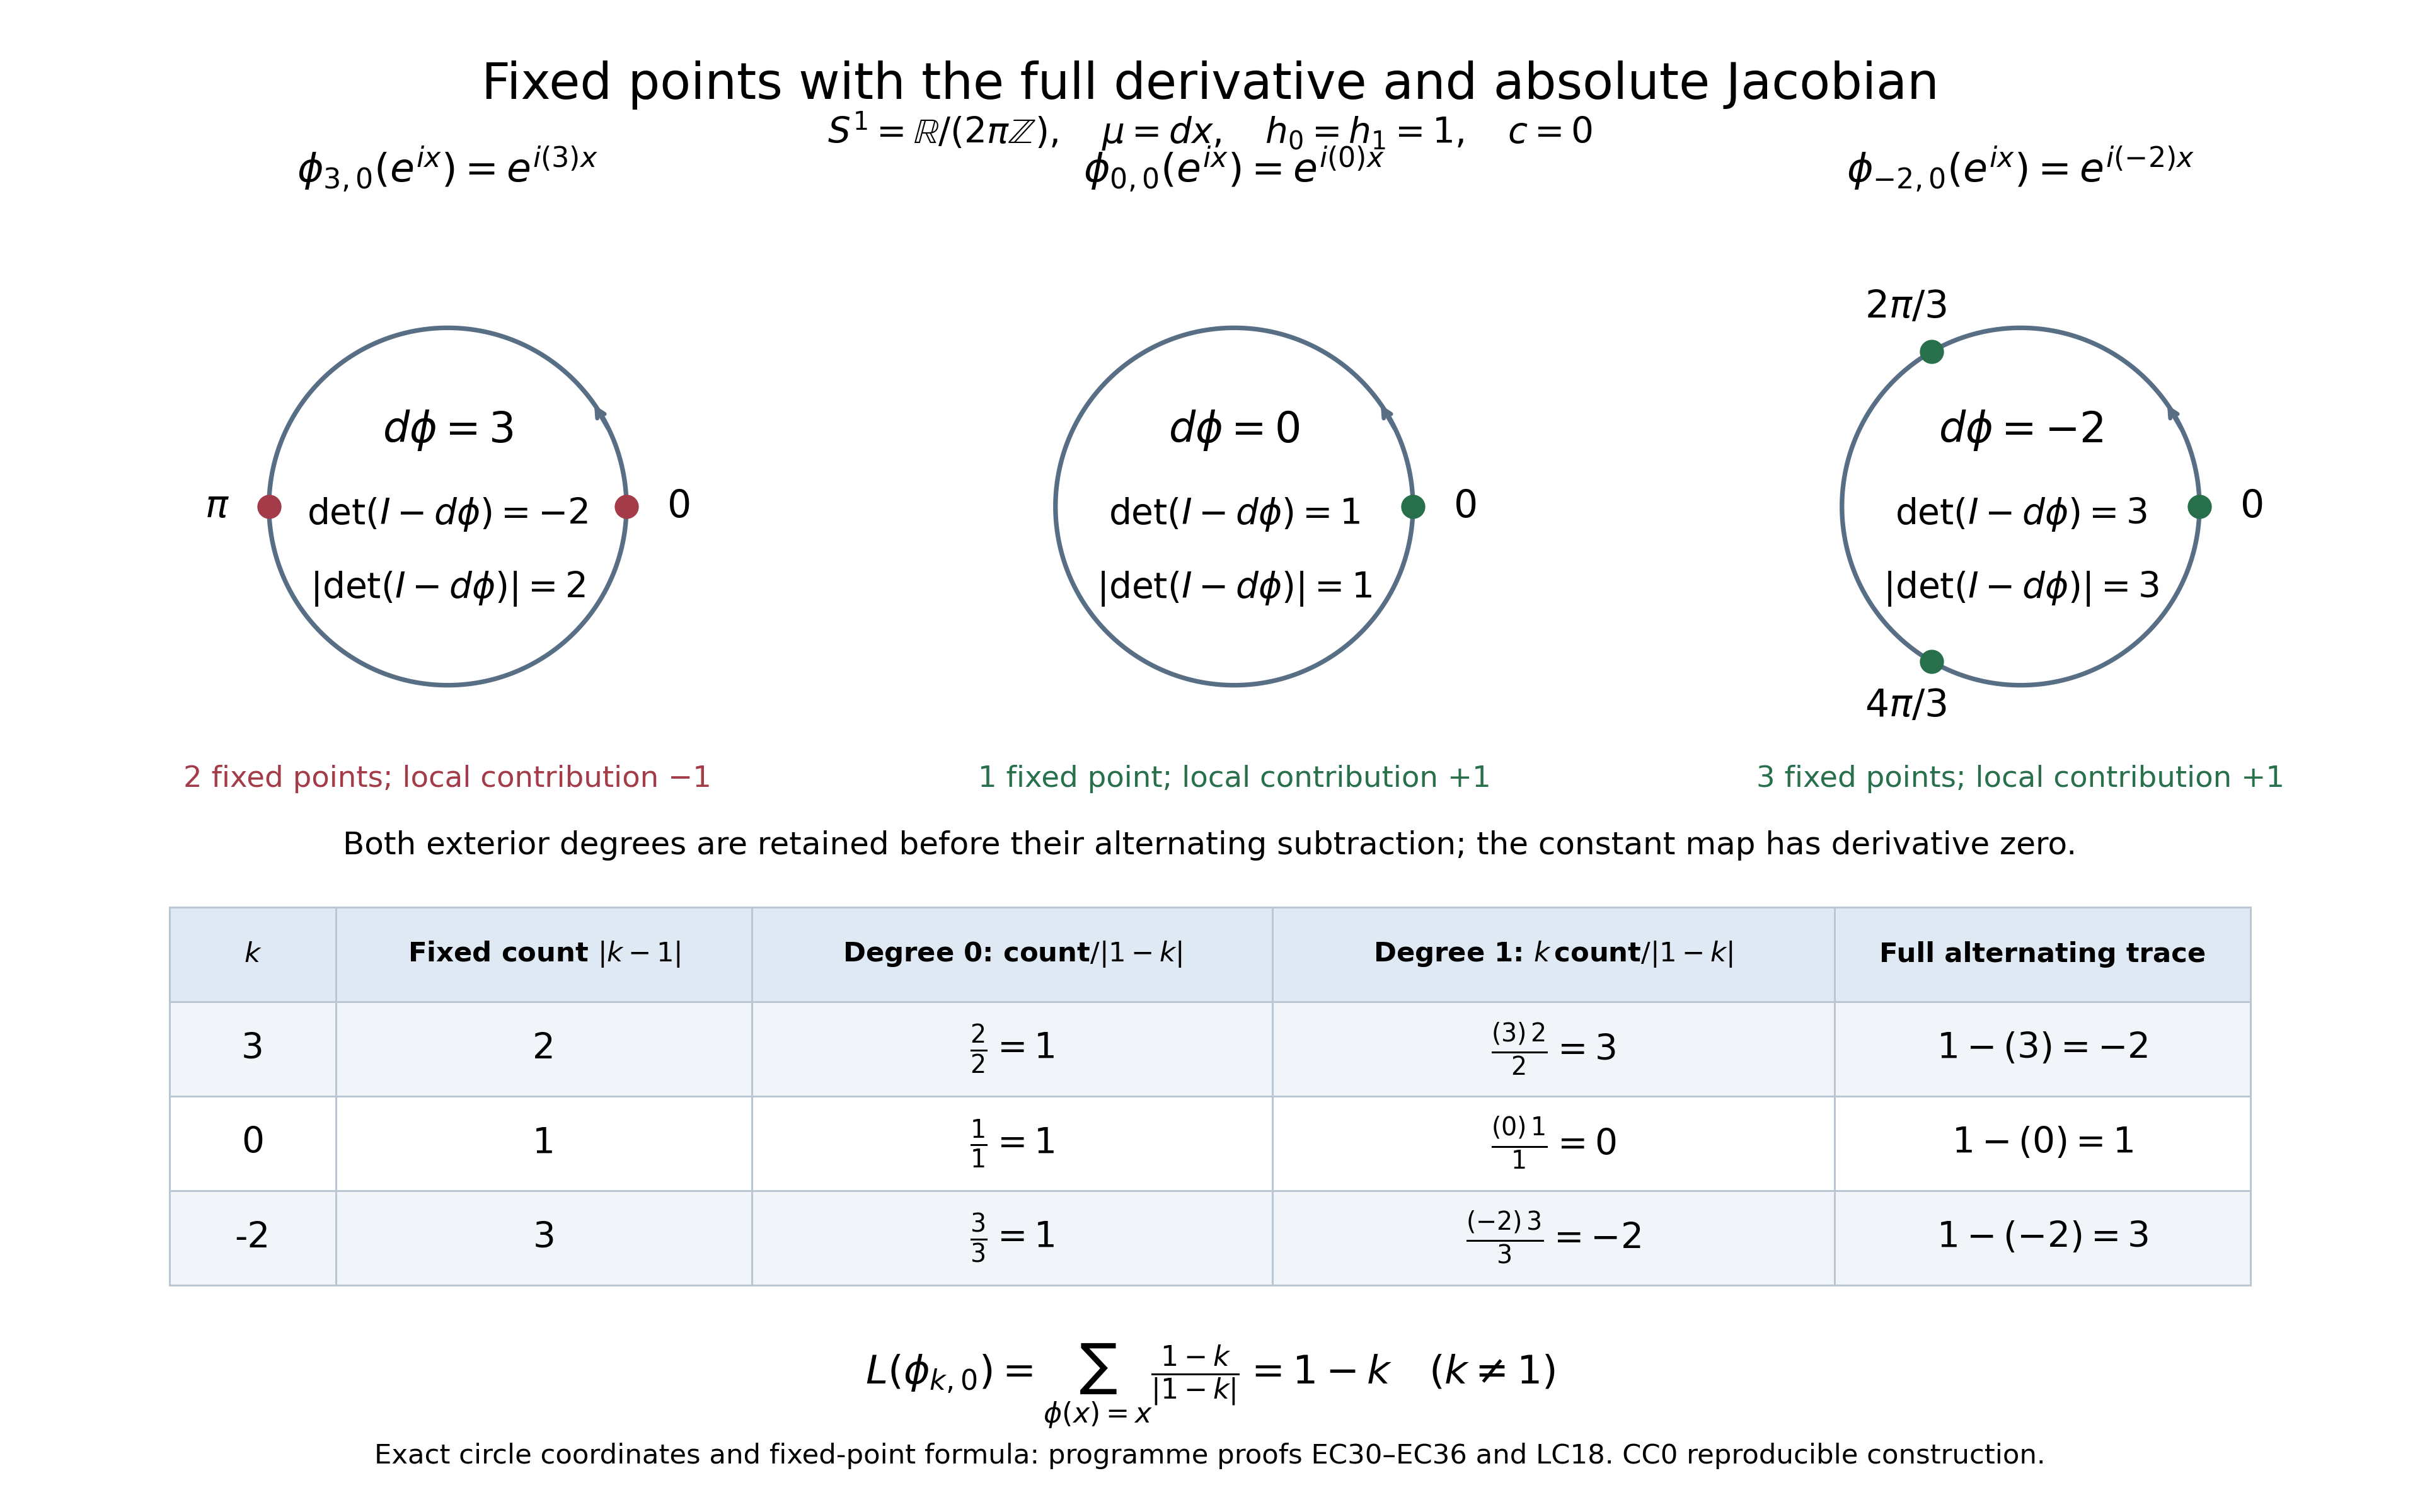
\includegraphics[keepaspectratio,alt={The exact circle fixed points and complete diagonal-trace factors for derivatives 3, 0 and −2}]{../figures/elliptic-complex-fixed-point-signs.png}}
\caption{The exact circle fixed points and complete diagonal-trace
factors for derivatives 3, 0 and −2}
\end{figure}

The figure uses the original circle angle modulo \(2\pi\), density dx,
unit displayed bundle frames and zero phase c.~The marked angles are the
exact fixed points of \(\phi_{3,0},\phi_{0,0},\phi_{-2,0}\), not
numerical zero estimates. The full derivative, signed determinant,
absolute determinant and both exterior-degree contributions remain
visible. The sampled curve depicts only the smooth unit-circle
embedding. Its reproducible source is
\href{../figures/elliptic-complex-fixed-point-signs.py}{elliptic-complex-fixed-point-signs.py},
and the complete proof is (EC30)--(EC36) and (LC18).

\subsection{14. The exact circle metric choice and its full weight
defect}\label{the-exact-circle-metric-choice-and-its-full-weight-defect}

The unit Fourier-frame computation in (EC37)--(EC38) uses the Hermitian
metrics for which the displayed frames 1 and dx are unit. A density
alone does not force these bundle metrics. Keep the original circle,
density dx, differential \ensuremath{\partial}\_x and half-density factor dx\^{}(1/2), but
now give those frames arbitrary positive smooth squared norms
h\_0(x),h\_1(x). The full integration-by-parts identity gives \[
D_0^*u=-h_0^{-1}\partial_x(h_1u),\qquad
\Delta_0f=-h_0^{-1}\partial_x(h_1\partial_xf),\qquad
\Delta_1u=-\partial_x\bigl[h_0^{-1}\partial_x(h_1u)\bigr].
\tag{LC19}
\] Its precise difference from the displayed unit-metric adjoint is
\(-(h_1/h_0-1)\partial_x-h_1'/h_0\); both coefficients are retained.
Thus a nonunit metric changes the original adjoint and both full
Laplacians, rather than being absorbed into the density. Positivity on
the compact circle gives all actual weighted L² bounds.

The energy kernels are K\_0={\ReaderSymbols\char"2102}·1 and K\_1={\ReaderSymbols\char"2102}·h\_1\^{}(−1), and the
complete projections are \[
H_0f=\frac{\int_0^{2\pi}h_0 f\,dx}{\int_0^{2\pi}h_0\,dx},
\qquad
H_1u=\frac{\int_0^{2\pi}u\,dx}{\int_0^{2\pi}h_1^{-1}\,dx}\,h_1^{-1}.
\tag{LC20}
\] Each formula follows by retaining the original weighted inner product
with its actual kernel generator and dividing by that generator's full
squared norm. Put \(v=u-H_1u\); its ordinary integral is exactly zero.
The actual degree-lowering primitive is \[
G_0u(x)=\int_0^xv(s)\,ds
 -\frac{\displaystyle\int_0^{2\pi}h_0(t)
                       \left(\int_0^tv(s)\,ds\right)dt}
        {\displaystyle\int_0^{2\pi}h_0(t)\,dt}.
\tag{LC21}
\] It is periodic because the full integral of v vanishes, and has zero
h\_0-weighted mean. Differentiation gives D\_0G\_0=I−H\_1. For u=D\_0f,
its degree-one harmonic part is zero by the periodic fundamental
theorem; (LC21) gives G\_0D\_0f=f−H\_0f. This is the original G\_0 from
(EC12): both solve the same derivative equation with the same harmonic
annihilator, and their difference is a constant with zero weighted mean.
For a mean-zero periodic distribution v define its actual Fourier
primitive \(Jv=\sum_{n\ne0}v_n(in)^{-1}e^{inx}\). Its coefficients
retain polynomial growth, hence define a distribution by the complete
test expansion in (LC8). It maps H\^{}s into H\^{}(s+1): the full
multiplier bound is \(\langle n\rangle/|n|\leq\sqrt2\) for every n\ensuremath{\ne}0.
The extension of (LC21) is exactly
\(Jv-(\int h_0Jv\,dx)/(\int h_0\,dx)\). On smooth inputs the base-point
constant in the integral from zero cancels in the weighted mean, proving
agreement with (LC21). Both weighted projections are smoothing and have
their full bounded distribution-smooth pairings, so this proves every
stated Sobolev and distributional extension directly. For h\_0=h\_1=1
every formula returns the exact original Fourier operators, including
1/(in), n\^{}(−2), the complete zeroth projection and every 2\ensuremath{\pi} factor.
The two harmonic spaces and Euler index stay unchanged through the
explicit comparison (LC13).

All strengthenings above have complete proofs for their written objects.
The source-reading ledger distinguishes exact earlier programme proof
reuse from new content reading and unread indexed literature. No
novelty, whole-course clearance or reader/source equality is claimed by
this supplement.

\end{document}
